\documentclass[12pt,oneside]{book}
\include{macros/style}

% Long Table and decimal aligned columns
\usepackage{dcolumn}
\usepackage{longtable}

% Mathematics support
\usepackage{amsmath}
\usepackage{amsthm}
\usepackage{amssymb}


% Text Control
\usepackage{xspace}
\usepackage{textcase}

% Graphics
\usepackage{wasysym}
\usepackage{graphics}
\usepackage{graphicx}
\usepackage{float}

% Algorithm
\usepackage{algorithm}
\usepackage{algorithmic}
\usepackage[T1]{fontenc}

% Define some commands for easy typing
\newcommand{\etal}{et al. }
\newcommand{\blob}{\textit{BlobTree }}
\newcommand{\blobns}{\textit{BlobTree}}

\begin{document}

% Front Matter
\input frontmatter/fm

\newpage

%The structure of my thesis break-down into several chapters. Each chapter relates to one phase of the project
	%\newcommand{\etal}{et al. }
%\newcommand{\blob}{\textit{BlobTree }}
%\newcommand{\blobns}{\textit{BlobTree}}


\startfirstchapter{Introduction}
\label{chapter:introduction}
\section{General aim of this Research}
Simulating the behavior of elastic objects in real time and with some level of user interaction is a challenging problem 
with many applications in different areas of research including virtual surgery \cite{Meier2005}. 
In computer graphics, the models used for the construction of objects with deformable behavior are known as deformable models. 
A complete model should be quite realistic, interactive and should enable the user to modify the topology of the objects.
Therefore, there exist a number of contrasting constrains: high fidelity, which in general implies accurate models and high frame rate,
and use of low cost computers. A number of proposals have been recently presented to fulfill these objectives. But even if the efficiency
of the simulation models have been largely improved in the last few years, soft object modelling and deformation remains a rather 
complex task and can be solved in interactive time only on models composed by a few hundreds of cells. In addition, integrating effects
such as cut and lacerations, makes the simulation model more complex. In modern interactive simulation and modelling environments the ability to 
cut 3-dimensional geometry in real-time is of fundamental importance. This creates the need for efficient cutting algorithms that process the 
underlying representation. In surgery simulation, interactive cutting algorithms enable the dynamic simulation of scalpel intersections that open 
immediately behind the scalpel \cite{Nienhuys2001}. Cutting a volumetric mesh under deformation is a non-trivial problem, due to several conflicting
requirements. On the one hand, the cutting process should not create badly shaped elements, which could cause numerical instabilities during deformation
calculation. On the other hand cut trajectory should be closely approximated for realistic appearance. So far, most methods have concentrated only on 
one of these problems. 

Therefore the following major problems are identified in the surgical simulation domain:

\begin{itemize}
 \item Modelling complex tissues that are readily available for simulation \cite{Nealen2006,Meier2005,Gibson1997a}.
 \item Real-time visualization of those tissues \cite{Mario2010PolygonMesh,Bloomenthal1997}.
 \item Performing interactive topological modifications on complex models while under deformation \cite{Jin2013,Wu2011,Courtecuisse2010a,Jerabkova2010}. 
\end{itemize}

We present a comprehensive solution to these problems as following. 
First, our proposed modelling solution captures the key advantages found in volumetric modelling approaches using 
implicit surfaces \cite{Bloomenthal1997, Wyvill1986, Wyvill1999, Wyvill1996, Wyvill1997, Schmidt2006, Bernhardt2010a}. Automatic blending and compact 
representation are the major benefits of using implicit surfaces for modelling. In addition, the ability to perform inside-outside tests 
easily is an inherent advantage in implicit models when implementing physically based simulations requiring collision tests. 
The \blob \cite{Wyvill1999} combined blending, affine transformations and constructive solid geometry (CSG) operators in a 
comprehensive and compact scene graph data-structure. \blob provides the ability to create complex models incrementally \cite{Schmidt2006}. 

Secondly we propose a solution for high performance and scalable visualization of complex models created by \blob method.
Volumetric models in general are often several orders of magnitude slower during visualization \cite{Bloomenthal1990a, Bloomenthal1997}.
We proposed a data-driven algorithm for rendering complex implicit models in real-time on multi-core processors \cite{Shirazian2012}, later, we 
fine tuned that algorithm for running on many core architectures such as the ones in high-end graphical processing units (GPUs). 

Third, we take a different approach to develop a stable and realistic cutting system. Our GPU-assisted interactive cutting algorithm allows
arbitrary cuts in the model and can enable many scenarios for tissue manipulation while under deformations. 

In what follows, the implicit modelling approach to deformable tissue design will be studied. To achieve the initial goal of this research, a
computational framework for designing, rendering and animating deformable tissues has been developed and the details of the process is documented 
in the following chapters. 


\section{Deformable Models}
Deformable models can be defined in either one dimension (lines and curves), two dimensions (surfaces), or three dimensions (solid objects). 
Essentially, they are applied in three different areas of research \cite{Meier2005}: 

\begin{itemize}
 \item Object modelling for pre-computed animations \cite{coquillart1990extended, hsu1992direct}.
 \item Image segmentation (automatic 2D interpretation of the images provided by a camera or 3D reconstruction of organs from medical MRI 
 or CT scans) \cite{neveu1994recovery}.
 \item Interactive medical simulations i.e. to emulate the deformational behavior of non-rigid objects due to external influences.
\end{itemize}

Our solution is targeted for the last area where it can be used both in deferred application like surgery planning (e.g., simulation of the 
outcome of craniofacial surgery) \cite{bro1995modelling, keeve1996craniofacial} and real-time applications 
including image guided surgery \cite{Szekely2000}, minimally-invasive or tele-surgery. 


There is no single deformable model that is appropriate for all of the above mentioned 
problems. Instead, there are a variety of methods that are optimized in different ways to meet specific 
needs. 
Current deformable model solutions trade precision in exchange with real-time response.
Even though real-time applications of deformable models are becoming more and more frequent, 
in many cases, the governing prerequisite for the simulation of 
mechanical deformations has been interactivity rather than precision. In addition to that, many of the modelled objects like garments or soft 
tissues do not possess easily describable properties. Consequently, other approaches must to be found 
\cite{bro1998finite}. Important progress in the field of deformable models has been made since the emergence of surgery 
simulation, with one of the first contributors being Cover et al. \cite{cover1993interactively}. 


% move to the section in background
This is mostly due to the extreme prerequisites 
as far as computation time, complex properties of the simulated soft tissues, and intricate interactions with the virtual instruments are concerned. 
In fact, there have been many different points of departure in the research of adequate deformable models, focusing on anatomies and surgical techniques 
that are as different from each other as are eye surgery \cite{cai2001parametric, sagar1994virtual}, knee arthroscopy \cite{gibson1997simulating, 
hoffman1998commercially}, or hepatic laparoscopy \cite{cotin1999real}. The deformable models developed in this context can be divided into three basic groups: 

\begin{enumerate}
 \item The ad-hoc heuristic methods
 \item Simplified continuum-mechanical model
 \item Hybrid methods from the combination of 1 and 2
\end{enumerate}



\section{Motivation}

%%these bits should go under requirements
Laparoscopic surgery brought new technologies into the operating room and created a 
distance between the surgeon and the patient. More recently, other minimally invasive techniques have 
been proposed, such as natural orifice transluminal endoscopic surgery, which can be considered as an 
evolution of laparoscopic surgery. Laparoscopy requires surgeons to acquire new skills, and adapt 
to changes from conventional open surgery e.g. amplified tremor, diminished tactile sensation, loss of 
depth perception.  Without open organ surgery, modern surgeons do not get 
training in the motor skills of the previous generation. Thus there is a 
motivation to develop realistic surgical simulations using 
real-time deformable models, and haptic rendering for further realism \cite{Lin2004}. 
The following benefits have been reported from 
using surgical simulation systems:  \cite{}

\begin{itemize}
 \item Systematic training and objective assessment of technical competence
 \item Skills learned thanks to the simulator are transferable to the operating room
 \item The ability to create patient-specific simulations (i.e. rare pathological cases or when the best surgical strategy is unclear.)
 \item The ability to use augmented reality for image-guided surgery (i.e. to improve the accuracy and limit the adverse effects of surgery)
\end{itemize}

%These are the benfits
In order to achieve these benefits, accurate, real-time bio-mechanical models are needed together
with interactions with medical devices. Such interactions involve tissue manipulation and tissue dissection. 

In this context, modelling and high-performance rendering of soft-tissues are the core requirements for 
a simulation scenario. The development of fast algorithms to compute the deformation, contact response, 
cutting and haptic feedback of soft tissues could enable a number of the aforementioned applications.


\section{Limitation of Current Models}
\label{sec:limitationsOfCurrentModels}
%%Requirements listed below and then 

The requirements listed below are considered in our design of a robust deformable 
model for surgical simulations:

\begin{itemize}
  \item Anatomical models and tissue properties need to be patient-specific and 
obtained without complex additional procedures
  \item Soft tissue behavior needs to be realistic and demonstrate a predictive capability, yet it should be 
  compatible with real-time computation
  \item Interactions with the surrounding anatomy and with medical devices need to involve advanced 
  contact models that can be computed in real-time
  \item The different types of dissection performed on soft tissues should be simulated
  \item Realistic visual and haptic feedback should be provided to create a higher level of immersion, in 
  particular during training sessions
\end{itemize}

%%Chapter \ref{chapter:background} will provide more details on the state of the art techniques in soft tissue modelling. 

%note to self
Among the existing approaches we can cite methods based on spring-mass networks, methods based 
on linear elasticity, and explicit finite element models for non-linear materials 
\cite{Gibson1997a,Meier2005}. In chapter \ref{chapter:background} we discuss these methods in detail.  

Mass-spring networks are quite simple to implement and very fast to compute, but they fail to properly 
characterize soft tissues deformation as they introduce artificial anisotropy through the choice of the 
mesh, and make it difficult to relate spring stiffness to material properties such as Young's modulus 
\cite{Courtecuisse2010}.

Most methods assume Linear elasticity based on small displacements and pre-computed 
response values to accelerate the computations. The small strain assumption is very restrictive. In 
addition, during any topological modifications e.g. in cutting, the pre-computed values 
have to be recalculated which masks their effectiveness in the overall performance of the system.

Cutting deformable tissues is one of the most sought after features in a surgical simulator. In an interactive 
system with high expectations of realism and performance, the implementation of topological 
modifications can become very complex. The proposed solutions suffer from smoothness of the cutting 
plane or slower solve time due to lots of extra nodes added to the system. In chapter 
\ref{chapter:Cutting} we review all the related work in this topic and present our high performance 
cutting algorithm which is built into our physically-based simulation system.


\section{Contributions}
\label{sec:contributions}
Contributions described in this thesis fall into four broad categories: a modelling system to create 
complex deformable tissues under the heading of the \blob; a high-performance subsystem for 
rendering; a high-performance topology modification algorithm to support cutting and a  
real-time Craniotomy simulation for neurosurgery simulation. The full contributions list is as 
following:

\begin{itemize}
 \item A comprehensive modelling framework supporting a broad set of skeletal implicit primitives, 
 sketched primitive objects, warping, blending, affine transformations and constructive solid geometry 
 operators in the compact \blob structure. Our framework also provides a software architecture for 
 physically-based animation of rigid and deformable models 
 
 \item An algorithm for interactive polygonization of implicit surfaces on multi-core architectures with SIMD instructions.
 \item An optimized GPU-assisted algorithm for high-performance polygonization of implicit surfaces on many-core architectures.
 \item A high-performance algorithm for volume discretization of \blob models which can generate tetrahedral mesh elements with respect to a triangular 
 surface mesh for finite element formulation.
 \item A high-performance algorithm for cutting rigid and deformable tissues interactively.
 \item Smooth cutting of complex volumetric meshes to avoid producing the jagged lines without the 
 need for a post-processing step.

 \item A mesh data-structure suitable for storing dynamic meshes on the GPU to 
 support realtime modifications during cutting
 \item A novel technique for collision detection using implicit fields which is 
 used in our system to detect the intersection of the scalpel tool with the volume mesh in realtime. 
 
  \item Real-time Craniotomy simulation for neurosurgery and biopsy simulations.
\end{itemize}


\section{Overview}
In the next chapter we start by providing background material on implicit modelling technique, the \blob scene-graph and the concept of sketch-based, incremental modelling.
We continue by reviewing the physics properties of the deformable tissues and cover some topics on continuum mechanics concepts and force models used in
our system to achieve non-linear deformations. Chapter \ref{chapter:cpuPoly} presents our rendering framework to visualize complex \blob models using multi-core 
architectures. Building on the outcomes of chapter \ref{chapter:cpuPoly}, the improved results are reviewed in chapter \ref{chapter:GPUDiscretization}. 
The discretization technique to convert a \blob model to a physical system is also given in this chapter. 

In Chapter \ref{chapter:Cutting} we present one of the main contributions of this thesis which is the high performance soft tissue cutting. After a brief overview of the 
related work we present our novel technique in cutting complex soft tissues interactively. Chapter \ref{chapter:evaluation} showcases a skull craniotomy simulation 
scenario and provides comments on the operation itself and the achieved results.

In Chapter \ref{chapter:conclusion} we provide a summary of the results in the previous chapters and reviews the limitations of the current system
and some discussions on the future work in this research topic.


In this research we take into account the requirements of modern surgical 
procedures and introduce a new real-time deformable model with the ability to 
perform real-time topological changes (cutting) in a non-linear model, providing 
more realistic behavior than has can be provided by existing models. 















	\startchapter{Background Material}
\label{chapter:background}

\newlength{\savedunitlength}
\setlength{\unitlength}{2em}
This chapter provides a short summary of the material which is relevant to the subject of this research. 
We describe the concepts underlying implicit modelling, CPU and GPU architectural differences and 
scalability issues. The chapter concludes with a review of the related work in this domain.

\section{Implicit Modelling}
\label{sec:implicitmodellingintro}
Parametric surfaces such as Bezier patches has a generative form that enables 
two dimensional iteration over the surface directly. However, in the case of implicit models, 
the surface is surrounded by the object's volume and an extraction process is required to 
access the boundary surface. The formal definition of the surface and volume in this case is as following:

\begin{equation}
S = \left\{M = (x,y,z) \in \mathbb{R}^3 | F(x,y,x) = c\right\}
\end{equation}

\begin{equation}
V = \left\{M = (x,y,z) \in \mathbb{R}^3 | F(x,y,x) \geq c\right\}
\end{equation}

Function $F$ computes the field value at a certain position $M$.  $c$ is a constant and is called the \textit{iso-value} 
which is set to $0.5$ in our system. For each point in space if the field is greater than $c$ the point is 
considered inside the model otherwise outside. 

Most of the primitives used in the \blob are built from geometric skeletons, which are incorporated in many implicit modelling software packages 
such as BlobTree.net \cite{Groot2008} or ShapeShop \cite{Schmidt2006}. They are ideally suited to prototype shapes of arbitrary topology 
\cite{Bloomenthal1997}. In general these works conclude that the use of skeletal primitives can lead to a simple and intuitive user modelling 
methodology. The basic building block of a skeletal primitive is a skeleton $S$. To create a skeletal primitive the distance-field $dS$ of the 
volume encapsulating the shape has to be computed as described in \cite{Barbier2004}. The distance field is a volume of scalar values which is 
not bounded as the distance itself can be infinitely large.

By modifying $dS$ with a field function $g$, it can be bound to a finite range. Usually the function maps the distances to the range $[0, 1]$, 
where the field has values of 1 at the skeletons and 0 after a certain distance to the skeleton (usually at distance 1). A discussion of field 
function is provided in \cite{shirley2009graphics}. Skeletal implicit primitives are combined 
using binary operators, which are applied pair-wise to field-values f, and represented by a 
node in the \blob, whose children are either primitives or operators themselves.

Field values are computed for the child-nodes and combined to yield a new value according 
to the operator type. This makes it possible to go beyond the classical Boolean operators, 
and define general blend operators that e.g. create smooth transitions between shapes. The 
most common operator that creates a smooth transition between several values is called the 
summation blend \cite{Bloomenthal1997}:

\begin{equation}
F_A(x, y, z)=\sum_{i=1}^{i=N_A}F_i(x, y, z)
\end{equation}

Where an implicit model $A$ is generated by summing the influences of $N_A$ skeletal elements: 
The field value due to an skeletal element at a point in 3D-space is computed as filtered distance to its skeleton 
where the filter function (i.e. falloff function) is defined as follows \cite{Wyvill1999}: 

\begin{equation}
g_\mathrm{wyvill}(x)= \left\{ \begin{array}{rl}
 1 &\mbox{ if $x\leq0$} \\
 (1-x^2)^3 &\mbox{ if $0<x<1$}\\
  0 &\mbox{ if $x\geq1$}  
  \end{array} \right.
\label{eq:WyvillFunc}
\end{equation}

In equation \ref{eq:WyvillFunc}, $x$ is clamped to the range $[0,1]$. This polynomial smoothly decreases from 1 to 0 over the valid range, with zero
tangents at each end. An important property of this skeletal primitive definition is that the scalar field is \textit{bounded}, meaning that $f=0$
outside some sphere with finite radius. Bounded fields guarantee local influence, preventing changes made to a small part of a complex model from
affecting distant portions of the surface. Local influence preserves a \textquotedblleft principle of least surprise\textquotedblright that is critical 
for interactive modelling.  

Normals can be derived from gradients which are computed by evaluating 4 field values and performing a numerical approximation:

\begin{equation}
\nabla F(x,y,z)=\left\{ \begin{array}{rl}
 F(x+\delta,y,z)-f \\
 F(x, y +\delta,z)-f \\
 F(x, y, z+\delta)-f \\
  \end{array} \right. 
\label{eq:Normal}
\end{equation}

Where $f = F(x,y,z)$ is the field at point $(x,y,z)$.
% $fv = F(x,y,z)$ be the field at a point:
%$\nabla F(x,y,z)=\frac{1}{\delta}\left( F(x+\delta,y,z)-fv \right)$

Each skeletal primitive has a bounded region of influence in space. For each node in the tree an
axis-aligned bounding box is computed which is used to trivially reject those field queries that 
are outside the box. The bounding box of the entire model is computed as the union of all primitive
nodes bounding boxes.

For evaluating the field  at a point $P$ in a \blob model such as the one shown in figure (\ref{fig:CoffeeMugBlobTree}), 
the tree structure should be traversed from root to leaves recursively. Each operator combines the values of its children 
according to its type. For example, for a simple blend the values are summed. A leaf node represents a primitive,  and 
returns the value by applying equation~\ref{eq:WyvillFunc} to the distance of $P$ from the primitive.

%The right way for inserting figures
\begin{figure}[H]
\centering
  % the following command controls the width of the embedded PS file
  % (relative to the width of the current column)
  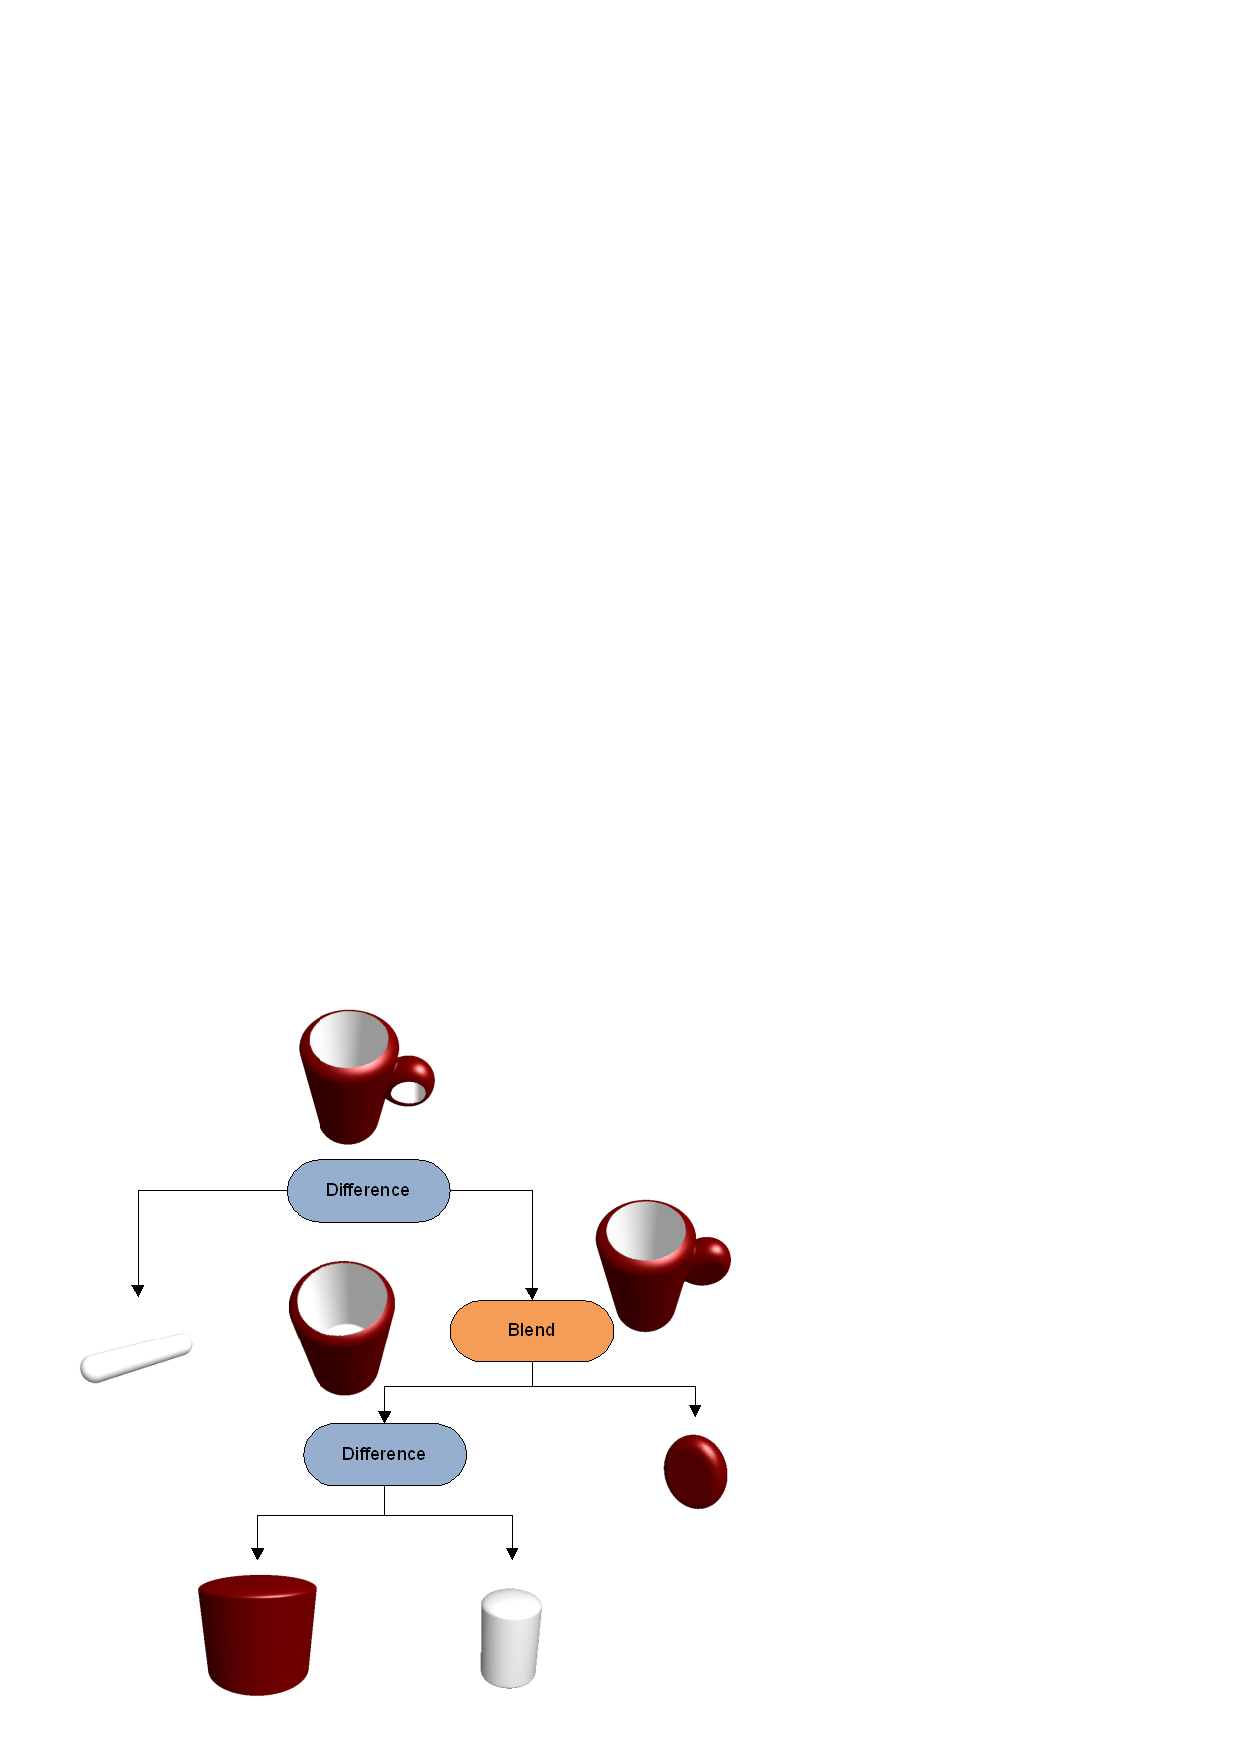
\includegraphics[width=1.0\linewidth]{figures/intro/CoffeeMugBlobTree}
  \caption{\blob structure of a coffee mug created with CSG and skeletal implicit primitives.}
  \label{fig:CoffeeMugBlobTree}
\end{figure}

%As the tree gets deeper and the number of primitives increase the computation 
For visualization purposes the \blob is queried numerous times to evaluate the field. As suggested in \cite{SWG2005} 
accelerating field computation will have a large impact on the overall surface extraction process. 

\section{Sweep Surfaces and Sketching}
Implicit primitives in our system are created from skeletons which are simple geometrical shapes such as points, line segments or 
polygons from which volumetric distance fields are created. In order to support more complex geometries \textit{Schmidt} \etal proposed the
implicit sweep objects technique where the 2D shape sketched by the user is sampled and an implicit approximation is created from 
the sample points \cite{Schmidtc}. This is done by fitting a thin-plate spline as a base shape to the sampled points using variational 
interpolation \cite{Turk1999}. One advantage of creating the base shape using variational interpolation is that the resulting implicit 
field is $C^2$ continuous, a property needed when the shape is involved in several blending operations \cite{barthe2004controllable}.

A continuous 2D scalar field is created from several field value samples $(\mathbf{m}_i, v_i)$, where $\mathbf{m}_i$ describes the 
position of the sample and $v_i$ is the desired field. The thin-plate spline used to create the variational 
implicit field $f_c(\mathbf{u})$ is defined in terms of these points weighted by corresponding coefficients $w_i$ combined with a polynomial 
$P(u) = c_1u_x +c_2u_y +c_3$.

\begin{equation}
f_c(\mathbf{u}) = \sum_{i \in N} w_i(\|\mathbf{u}-\mathbf{m}_i\|)^2ln(\|\mathbf{u}-\mathbf{m}_i\|)+P(\mathbf{u}) 
\label{eq:thinplatespline}
\end{equation}

The weights $w_i$ and coefficients $c_1$, $c_2$, and $c_3$ are found by solving a linear system defined by evaluating 
equation \ref{eq:thinplatespline} at each known solution $f_c(\mathbf{m}_i)=v_i$.
The resulting thin plate spline can then be used as the basis of several different primitives:

\begin{itemize}
 \item Inflated Objects
 \item Swept object along a trajectory
 \item Revolving object around axis
\end{itemize}

These sketched objects can then be used in the same way as the standard skeletal implicit primitives to create unique 3D shapes. Such 
unique shapes were not possible to create in previous collaborative environments, especially given the small memory footprint 
needed to transfer the information when using this technique.



%-------------------------------------------------------------------------
\section{Related Work}
\label{sec:relatedwork}

In the following we review the related work associated with the major contributions of our research. 
The surface extraction methods that attempted to enhance the performance of the 
sampling process on multi-core CPU processors are reviewed first. Some others attempted to exploit the processing 
power on the GPU and mapped the same problem to many-core processors. Later 
the previously proposed algorithms for cutting volumetric meshes and the application of this framework 
in a surgical simulation (Craniotomy) are studied. 


\subsection{Surface extraction methods}
Several methods for polygonization of implicit surfaces have been proposed which can be 
classified based on speed, accuracy of the output mesh or quality.  Comparing these methods in terms of performance reveals that space 
partitioning methods are the fastest and the most popular. The paper \cite{Wyvill1986} was the first to introduce a method for finding 
iso-surfaces using uniform space subdivision into cubic cells. A seed cell on the surface was found by starting at a vertex close to 
each primitive and evaluating the field at cell vertices along each of the three axes to find a surface crossing. Vertices inside the 
volume were classified as `hot' and `cold' outside. A hash table was used to keep track of processed cells to avoid redundant field 
evaluations and to avoid storing any cells that did not contain part of the surface. Only adjacent cells that share an intersecting edge 
with their parent were processed, and a second cubic subdivision served to reduce the number of primitives considered in each field evaluation. 
Ambiguous cases were ameliorated by taking another sample from the center of the face.
A similar method was later introduced as Marching Cubes in \cite{Lorensen1987}. The main difference between the two algorithms was that 
Lorenson \etal applied their method to discrete volume data instead of sampling a continuous function and in Lorenson's method
the space was completely partitioned into cubic voxels and all cubes were visited.

Bloomenthal showed that the ambiguous cases can be dealt with by subdividing cells into tetrahedra \cite{Bloomenthal1994a}, and also 
that a six tetrahedron subdivision was superior to subdividing into five \cite{guziec1995exploiting}. 
The fact that tetrahedral simplices have 4 vertices reduces the total number of configurations to 16 (or 3 by symmetry), however, the number of 
redundantly generated triangles as a result of this decomposition increases significantly. 
We will refer to marching cubes and tetrahedra, with MC and MT respectively throughout this chapter.

%4. Serial Ehancements to MT and MC
There have been many enhancements proposed for both MC and MT. Some gain advantage by classifying cubes according to different criteria
and surface edge intersection calculation and number of field function evaluations. 
For example, Dietrich \etal \cite{Dietrich2009}, did a statistical analysis of cube configurations in MC that are responsible for most 
of the degenerate triangles in the output mesh. Their algorithm avoids those cube configurations by inserting an extra vertex into the 
cell when generating triangles as was done in \cite{Wyvill1986} where an extra sample was taken.
This reduces the statistical occurrence of the problem.

Triquet \etal \cite{Triquet2003} enhanced MT by applying time-stamps on calculated values and using hash tables for retrieving them. They
also pre-computed surface vertices along crossing edges which are shared with adjacent voxels and referenced previously calculated
values to avoid re-evaluating them. This latter enhancement was also done in Bloomenthal's polygonizer \cite{Bloomenthal1994a}
and was a fairly common feature of implicit surface polygonizer's of the 1990s.

%5. Parallel Enhancements on CPU
Beside enhancing serial algorithms some attempts were made to increase the performance of MC by dividing the workload between
multiple CPUs or on a network grid of computers. Mackerras proposed an MIMD implementation of MC algorithm \cite{mackerras1992fast}. 
The bounding volume is divided into uniform blocks and each processor runs a serial implementation of MC on one or more blocks. They 
reported that because of efficient usage of cache their method showed a speed-up greater than the total number of physical
processors involved. Hansen and Hinker presented a parallel implementation of MC \cite{hansen1992massively}. They labeled each cube
with a virtual processor identifier to avoid complexities in communicating between processors, then each cube is processed
independently. They reported linear speed-up by increasing the number of physical processors. Their method spends constant time on
each processor regardless of the number of polygons in a cubic cell.

%6. GPU polygonizers
The advent of shader programs and GPGPU computing interested some to port serially computationally intensive programs to the GPU. 
Space partitioning methods like MC and MT are good candidates for these devices since each cell (either tetrahedra or
cube) can represent an independent volume to be processed on a separate SIMD core. 

%Kipfer and Westerman paper
Kipfer and Westermann proposed a GPU-accelerated Marching Tetrahedra algorithm that stores the topology of the
surface on the GPU \cite{Kipfer2005}. They used a span-space interval tree to cull tetrahedral elements that don't intersect with the 
surface. Caching edge-surface intersections helped them to avoid redundant calculations. For computing edge-surface intersections they used
linear interpolation for finding roots along each edge which is less accurate and degrades the quality of the output mesh.  

%Johansson paper
Johansson \etal accelerated iso-surface extraction using graphics hardware \cite{Johansson2006}. They stored MC cases on the GPU 
and used a vertex program to compute surface intersection points. They used a span-space data-structure similar to \cite{Cignoni1997} to
enhance the cell classification phase in MC. Their method shows a speedup order of 13 over the naive algorithm.  


% DirectX$^{\textregistered}$ 10 is not needed
Tatarchuk \etal presented an iso-surface extraction algorithm implemented using DirectX \cite{Tatarchuk2008}. They used graphics 
hardware to visualize medical data. They maximized utilization of SIMD units on the GPU by separating their polygonization (which is a 
hybrid of marching cubes and marching tetrahedra) into two phases: Fast cube tetrahedralization and a marching tetrahedra pass. Each input 
voxel position is dynamically computed in the vertex shader, then they used the geometry shader and stream-out features of DirectX 10 to 
tessellate voxels into six tetrahedra spanning the voxel cube. However their method is limited to medical volume datasets.

%Parallel Polygonization
An adaptive parallel polygonization method is proposed by Yang \etal \cite{Yang2010}. They enhanced the Araujo's method 
\cite{Rodriguesdearaujo2005} by dividing the bounding box of the model into eight parts and then processing them in parallel.
For each part, their method find a seed point on the surface and increasingly expand it to form a 
local mesh for the part by using the surface tracking approach. Using local curvature of the implicit 
surface, their method produces triangles of varying sizes. However, their method is not scalable since 
it can not guarantee finding a seed point per each sub box in case the number of sub boxes increases. 
They reported very slow rendering times even for the simple models that they have tested their system with. 


In a similar work Knoll \etal \cite{Knoll2007} proposed interactive raytracing of arbitrary implicits with 
SIMD interval arithmetic. They used SSE instructions for fast computation of interval arithmetic 
and ray traversal algorithm. However, their method is restricted to static implicit functions and 
algebraic surfaces.

None of the proposed methods above used a modelling framework to define their input data in a hierarchical structure similar to 
the \blobns. Their method is either limited to volume data or an algebraic implicit function to represent the underlying volume. 
In a closely related work, Schmidt \etal \cite{SWG2005} used a field caching mechanism inside the \blob to perform fast potential field 
reconstruction without traversing the entire tree. They used a trilinear reconstruction filter for field value and a triquaratic filter
for gradient interpolation. They evaluated cache efficiency by polygonizing a \blob model once using cache nodes and the other time 
without. They reported up to 16 times speedup for polygonizing a model with different resolutions. However, their method is not scalable since 
the cache nodes cannot be updated from different processing threads without using locking
mechanisms or a data race condition can occur. 

\subsection{GPU-Accelerated rendering of implicits}
GPU accelerated rendering techniques has been the topic of interest for the graphics community in the past two decades.
Several GPU-accelerated algorithms have been proposed for fast triangulation and rendering of iso-surfaces that are defined by
volume data-sets, algebraic surfaces and radial-basis functions. In this section we will review the most related works.

Chochl{\'i}k \etal proposed a GPU accelerated polygonization algorithm for dynamically changing implicit surfaces \cite{chochlik2012gpu}. 
Their method is based on the marching tetrahedra (MT) algorithm. The model is partitioned into cubic cells first and then each cell is 
subdivided into 6 tetrahedra to be further processed using the GPU geometry shading stage. The vertices are marked inside if their 
associated field is above zero and outside otherwise. A configuration index is computed per each tetrahedra based on the inside/outside 
vertices. The triangle mesh is produced which is shaded using the fragment shader stage. No further analysis has been made on the performance 
of their algorithm and the input models are limited to time varying simple algebraic surfaces. The used a linear interpolation root finding
method which produces low quality output. 

Buatois \etal proposed a GPU accelerated iso-surface extraction method based on MT, similar to Chochl{\'i}k \etal \cite{Buatois2006}. The 
texture memory to transfer the position and field values of the grid vertices. They presented an analysis of the performance of their algorithm
using a fluid simulation volume data-set. They reported that excessive texture fetches can be a bottleneck in the performance of their method.


Tatarchuk \etal proposed a GPU iso-surface extraction algorithm which is a hybrid of marching cubes and marching tetrahedra \cite{Tatarchuk2007}. 
They start by voxelizing an implicit grid into discrete cube cells and then convert that to a tetrahedral representation. They implemented an MT 
algorithm on geometry shader stage of DirectX10 API. For root finding method they fitted a parabola along the intersecting edges and evaluated a 
quadratic equation which produces a better approximation. They tested their system using the visible human volume data-set. Their method
is limited to static volume datasets and is not usable in a data-driven setting where the topology of the underlying model changes. 

With modern hardware and fast GPUs, ray tracing of implicit surfaces is the subject of much research. Knoll \etal \cite{Knoll2009} presented 
CPU and GPU algorithms that can achieve interactive visualization for common algebraic surfaces. The surfaces used in by Knoll \etal are not 
arbitrary implicit models but surfaces generated using traditional kernels or functions. Similar surfaces are presented by Singh and Narayanan
for real-time ray tracing of implicit surfaces using the GPU \cite{singh2010real}. 


Kipfer and Westermann \cite{Kipfer2005} accelerated rendering of implicit surfaces by avoiding redundant computation of edge surface intersections. 
Our method also employs this feature to reduce the overhead. They also use features of the GPU to reformulate the iso-surface identification and reduces 
numerical computations and memory access operations. They used a span-space data-structure to avoid processing non surface intersecting elements.

Kanai \etal \cite{Kanai2006a} proposed a rendering method for sparse low-degree implicit surfaces (SLIM) using ray casting approach. The ray and IS intersection
test has been carried out on the fragment processing stage. They employed level of detail rendering and view frustum culling to speedup the rendering. 
The coefficients for the IS are passed in using textures. They reported high quality and interactive rates for several models. The large number of processed
fragments is the bottleneck in this process and models with lower number of nodes could be rendered slower than more complex models that cover less fragments.
Although Kanai \etal's work is data-driven but the increasing cost of fragment processing is the main bottleneck in their system. Also since they are not
producing any mesh the computations will be lost after rendering.

\subsection{Volume mesh cutting}
A number of approaches has been proposed by the computer graphics community to enable cutting of deformable and rigid models. 
Except for a few methods most of them use tetrahedral meshes for the volumetric mesh representation. 
Bielser \etal performed an adaptive refinement of the tetrahedral elements cut by a virtual scalpel \cite{Bielser1999}.
In another work Bielser \etal presented a progressive approach to cutting \cite{Bielser2003}, where the decomposition of 
a tetrahedron is changed depending on the movement of the cutting tool inside an element. However, the approach is highly 
non-trivial to implement and also poses some stability problems due to badly-shaped elements.

Mor \etal tried to reduce the number of sub-elements created while cutting tetrahedral meshes \cite{Mor2000}.
One of the major issues in cutting is the creation of ill-shaped elements i.e. skinny elements, which can adversely affect the
performance and stability of the system solver. Some work attempted to avoid such elements via mesh alignment techniques 
\cite{Nienhuys2001b, Steinemann2006}. Other methods tried to solve the issue by removing them completely which resulted in 
volume loss and jagged lines along the cut surface. 

 
Wu \etal \cite{Wu2011} proposed an algorithm for 3D mesh cutting using a combination of the adaptive octree refinement with an iterative composite
element hierarchy to enable simulating high-resolution cuts with a small number of degrees of freedom (DOFs). 
They used the dual contouring method \cite{Ju2002} to keep the sharp creases along the cut. Due to the high computational cost and naive implementation 
their method is not scalable and has yet to become an interactive cutting approach.

In a closely related work Courtecuisse \etal presented a soft-tissue cutting system with haptic 
feedback \cite{Courtecuisse2010}. Their cutting strategy follows Mor \etal  \cite{Mor2000} work and 
suffers from jagged lines along the cut surface as shown in their examples of a laparoscopic hepatecotomy.
Progressive cutting, a feature that enables cutting the volume elements as soon as they become in contact with 
the scalpel, is not supported in their system and as most of the other works in this area they produce too many
new nodes when subdividing cut elements.

Jerabkova \etal proposed a solution to the ill-shaped elements problem by using hexahedral elements instead of 
tetrahedra \cite{Jerabkova2010}. Their approach relies on fine-level voxels to model object surface and simulate cutting. 
The volume data requires more memory space than traditional, surface-based models. Cutting is performed by
removing voxels. For sufficiently small voxels this typically remains unnoticeable but it may result in 
significant volume loss in case of a large number of cuts. 

Jin \etal proposed a meshless total Lagrangian adaptive dynamic relaxation cutting algorithm to predict the steady-state 
responses of soft tissue \cite{Jin2013}. A cloud of points is used for discretization and approximation of the deformation 
field within the continuum without generation of finite element meshes. They didn't report any performance measurements 
and the quality of the cuts could not be verified with the simple truth cube model they reported in their paper.

Sifakis \etal \cite{Sifakis2007} proposed a geometric algorithm for placing cracks and incisions on 
tetrahedralized deformable objects. Their method is similar to the virtual node algorithm in that they avoid 
sliver elements and their associated stringent timestep restrictions. Producing ill-conditioned triangles on 
the material surface can have a negative effect on collision handling specially in case of a self collision.
Also in their system a cut that partially intersects a tetrahedron without separating it into disconnected 
fragments will not allow the material to separate within that embedding tetrahedron.

Steinemann \etal \cite{Steinemann} created a hysteroscopy simulator and minimized the number of added elements 
after a tetrahedral subdivision by cutting along existing edges and faces. The problem with their system is that
the result of the cutting is produced only after it has been completed and this leads to a delay in the system. 
Unfortunately they didn't report any performance statistics of their algorithm. 

In the following sections we provide an overview of the system and the data structures involved in the process 
and our cutting algorithm. The chapter is concluded by the analysis of the simulation results.

\subsection{Applications in Surgical Simulation}
Abe \etal fabricated plastic skull models of seven individual patients by stereolithography from three-dimensional
data based on computed tomography (CT) bone images \cite{Abe1998}. Surgical approaches and areas of craniotomy were 
evaluated using the fabricated skull models. They reported a better understanding of anatomic relationships, preoperative
evaluation of the proposed procedure and improved educational experiences for the residents and medical staff as the benefits of 
their system. They also reported that the time and cost of making such models are the main disadvantages of using them.

Wong \etal loaded patient specific CT scans of cranial bone and CT angiography of intracranial circulation
into the Dextroscope workstation supplied by Volume Interactions Pte. Ltd \cite{Wong2007}. They showed various 
use-cases of the zoom, rotate, move and crop functions of the Dextroscope to visualize various angles of 
positioning the craniotomy. However, their system does not provide a physically-based simulation of the procedure. 

Stadie \etal performed a study on the effectiveness of virtual reality systems for placing the craniotomies 
in minimally invasive procedures \cite{Stadie2011}.  They used the Dextroscope and RadioDexter workstations 
supplied by Volume Interactions Pte. Ltd. to visualize and annotate the 3D VR models. 
Those systems are also used to measure the curvilinear distances of the proposed craniotomy centers on the 
patients skull model but they can not perform a cutting procedure on the input VR models.



\setlength{\unitlength}{\savedunitlength}

	\startchapter{High Performance Rendering on Multi-Core Architectures}
\label{chapter:cpuPoly}
One of the main challenges in animating deformable tissues is their rendering which requires to support high frame-rates \cite{Shirazian2012}. 
In order to leverage the benefits offered by \blob modeling the rendering issue has to be tackled accordingly. In this chapter
we present a parallel method for speeding up the generation of a polygon mesh from an implicit model \cite{Shirazian2012}. Although the method is applicable 
to many types of implicit surfaces, we focus on surfaces generated from fields surrounding geometric  primitives,  known as skeletal implicit 
surfaces,  \cite{Bloomenthal1997} that are discussed in chapter \ref{chapter:background}. The model data structure is a tree whose leaf nodes 
are primitives, and internal nodes are operators;  the \blobns, ~\cite{Wyvill1999}.
Currently the \blob supports operations such as;  arbitrary blends, boolean operations, warping at a local and global level including contact deformations. 
Geometric transformation matrices are also stored as nodes in the tree so the data structure is also a scene graph. 

A \blob  is typically visualized by  polygonization to produce a triangle mesh to be
rasterized by the graphics processor.  Direct ray tracing  \cite{Bloomenthal1997} can also be used,
to produce high quality images.  Both methods require computation of the field value which can 
only be evaluated by traversing the \blob structure. The field due to each operator depends 
on its child nodes and the leaves are the primitives which can be any implicitly defined function; 
e.g. distance field due to geometric skeletal elements.

Implicit  modeling using the \blob has several advantages  over other modeling methods.  Various different blends are simple to represent, 
as are free-form volume deformations and constructive solid geometry operations  (CSG) \cite{gomes2009implicit}. Other operators 
 such as detecting contact, and warping surfaces accordingly (see  \cite{Grascuel1997}),  can easily be represented as nodes in the \blobns. 

 An incremental, sketch based \blob system was built by Schmidt \etal \cite{Schmidt2006}, promoting flexibility and modular design for the creation of complex models, 
and most of the earlier problems with the methodology have been overcome \cite{Bernhardt2010a}. Although direct manipulation 
is possible  \cite{Schmidt2006},  very complex models can only be visualized interactively as coarse meshes. 
Hence the need for a faster polygonizer. The \blob facilitates incremental modeling, a strategy that promotes flexibility and modular design 
for creating  complex models. 

The main contribution presented here is a high performance polygonization algorithm that scales well with the 
number of physical cores and SIMD vector width available on modern processors.

As opposed to previous work that attempted to render implicit surfaces defined by static algebraic surfaces or 
volumetric scanned data, our method is data-driven where the definition of the surface can change over time. This feature 
is particularly useful in collision detection applications such as surgical simulations where the interaction
of the surgical tools and deformable tissues should be visualized in real-time \cite{Laycock2007}. 
 
In addition we have improved the performance of the algorithm that finds the intersection of a cube edge and the surface, by making use of the SIMD architecture, 
to find the intersection in a single run of a field evaluation kernel.


%We have tested our algorithm on two different processors with various number of cores and cache memory. 
The chapter is organized as follows;   related work is reviewed in section \ref{sec:relatedwork}, background information on implicit surfaces, 
skeletal primitives and the polygonization process is given in section \ref{sec:background}. In sections \ref{sec:algorithm} our algorithm 
is explained along with the improvements made to the distance-field computation process. Our performance results and future work are presented 
in sections \ref{sec:results} and \ref{sec:futurework}, respectively.

%-------------------------------------------------------------------------
\section{Related Work}\label{sec:relatedwork}
Several methods for polygonization of implicit surfaces have been proposed which can be 
classified based on speed, accuracy of the output mesh or quality.  Comparing these methods in terms of performance reveals that space 
partitioning methods are the fastest and the most popular. The paper \cite{Wyvill1986} was the first to introduce a method for finding 
iso-surfaces using uniform space subdivision into cubic cells. A seed cell on the surface was found by starting at a vertex close to 
each primitive and evaluating the field at cell vertices along each of the three axes to find a surface crossing. Vertices inside the 
volume were classified as `hot' and `cold' outside. A hash table was used to keep track of processed cells to avoid redundant field 
evaluations and to avoid storing any cells that did not contain part of the surface. Only adjacent cells that share an intersecting edge 
with their parent were processed, and a second cubic subdivision served to reduce the number of primitives considered in each field evaluation. 
Ambiguous cases were ameliorated by taking another sample from the center of the face.
A similar method was later introduced as Marching Cubes in \cite{Lorensen1987}. The main difference between the two algorithms was that 
Lorenson \etal applied their method to discrete volume data instead of sampling a continuous function and in Lorenson's method
the space was completely partitioned into cubic voxels and all cubes were visited.

Bloomenthal showed that the ambiguous cases can be dealt with by subdividing cells into tetrahedra \cite{Bloomenthal1994a}, and also 
that a six tetrahedron subdivision was superior to subdividing into five \cite{guziec1995exploiting}. 
The fact that tetrahedral simplices have 4 vertices reduces the total number of configurations to 16 (or 3 by symmetry), however, the number of 
redundantly generated triangles as a result of this decomposition increases significantly. 
We will refer to marching cubes and tetrahedra, with MC and MT respectively throughout this chapter.

%4. Serial Ehancements to MT and MC
There have been many enhancements proposed for both MC and MT. Some gain advantage by classifying cubes according to different criteria
and surface edge intersection calculation and number of field function evaluations. 
For example, Dietrich \etal \cite{Dietrich2009}, did a statistical analysis of cube configurations in MC that are responsible for most 
of the degenerate triangles in the output mesh. Their algorithm avoids those cube configurations by inserting an extra vertex into the 
cell when generating triangles as was done in \cite{Wyvill1986} where an extra sample was taken.
This reduces the statistical occurrence of the problem.

Triquet \etal \cite{Triquet2003} enhanced MT by applying time-stamps on calculated values and using hash tables for retrieving them. They
also pre-computed surface vertices along crossing edges which are shared with adjacent voxels and referenced previously calculated
values to avoid re-evaluating them. This latter enhancement was also done in Bloomenthal's polygonizer \cite{Bloomenthal1994a}
and was a fairly common feature of implicit surface polygonizer's of the 1990s.

%5. Parallel Enhancements on CPU
Beside enhancing serial algorithms some attempts were made to increase the performance of MC by dividing the workload between
multiple CPUs or on a network grid of computers. Mackerras proposed an MIMD implementation of MC algorithm \cite{mackerras1992fast}. 
The bounding volume is divided into uniform blocks and each processor runs a serial implementation of MC on one or more blocks. They 
reported that because of efficient usage of cache their method showed a speed-up greater than the total number of physical
processors involved. Hansen and Hinker presented a parallel implementation of MC \cite{hansen1992massively}. They labeled each cube
with a virtual processor identifier to avoid complexities in communicating between processors, then each cube is processed
independently. They reported linear speed-up by increasing the number of physical processors. Their method spends constant time on
each processor regardless of the number of polygons in a cubic cell.

%6. GPU polygonizers
The advent of shader programs and GPGPU computing interested some to port serially computationally intensive programs to the GPU. 
Space partitioning methods like MC and MT are good candidates for these devices since each cell (either tetrahedra or
cube) can represent an independent volume to be processed on a separate SIMD core. 

%Kipfer and Westerman paper
Kipfer and Westermann proposed a GPU-accelerated Marching Tetrahedra algorithm that stores the topology of the
surface on the GPU \cite{Kipfer2005}. They used a span-space interval tree to cull tetrahedral elements that don't intersect with the 
surface. Caching edge-surface intersections helped them to avoid redundant calculations. For computing edge-surface intersections they used
linear interpolation for finding roots along each edge which is less accurate and degrades the quality of the output mesh.  

%Johansson paper
Johansson \etal accelerated iso-surface extraction using graphics hardware \cite{Johansson2006}. They stored MC cases on the GPU 
and used a vertex program to compute surface intersection points. They used a span-space data-structure similar to \cite{Cignoni1997} to
enhance the cell classification phase in MC. Their method shows a speedup order of 13 over the naive algorithm.  


% DirectX$^{\textregistered}$ 10 is not needed
Tatarchuk \etal presented an iso-surface extraction algorithm implemented using DirectX \cite{tatarchuk2008advanced}. They used graphics 
hardware to visualize medical data. They maximized utilization of SIMD units on the GPU by separating their polygonization (which is a 
hybrid of marching cubes and marching tetrahedra) into two phases: Fast cube tetrahedralization and a marching tetrahedra pass. Each input 
voxel position is dynamically computed in the vertex shader, then they used the geometry shader and stream-out features of DirectX 10 to 
tessellate voxels into six tetrahedra spanning the voxel cube. However their method is limited to medical volume datasets.

%Parallel Polygonization
An adaptive parallel polygonization method is proposed by Yang \etal \cite{Yang2010}. They enhanced the Araujo's method 
\cite{Rodriguesdearaujo2005} by dividing the bounding box of the model into eight parts and then processing them in parallel.
For each part, their method find a seed point on the surface and increasingly expand it to form a 
local mesh for the part by using the surface tracking approach. Using local curvature of the implicit 
surface, their method produces triangles of varying sizes. However, their method is not scalable since 
it can not guarantee finding a seed point per each sub box in case the number of sub boxes increases. 
They reported very slow rendering times even for the simple models that they have tested their system with. 


In a similar work Knoll \etal \cite{Knoll2007} proposed interactive raytracing of arbitrary implicits with 
SIMD interval arithmetic. They used SSE instructions for fast computation of interval arithmetic 
and ray traversal algorithm. However, their method is restricted to static implicit functions and 
algebraic surfaces.

None of the proposed methods above used a modeling framework to define their input data in a hierarchical structure similar to 
the \blobns. Their method is either limited to volume data or an algebraic implicit function to represent the underlying volume. 
In a closely related work, Schmidt \etal \cite{SWG2005} used a field caching mechanism inside the \blob to perform fast potential field 
reconstruction without traversing the entire tree. They used a trilinear reconstruction filter for field value and a triquaratic filter
for gradient interpolation. They evaluated cache efficiency by polygonizing a \blob model once using cache nodes and the other time 
without. They reported up to 16 times speedup for polygonizing a model with different resolutions. However, their method is not scalable since 
the cache nodes cannot be updated from different processing threads without using locking
mechanisms or a data race condition can occur. 

A background on implicit surfaces and \blob modeling is provided in section (\ref{sec:implicitmodelingintro}) in chapter \ref{chapter:background},
which will be helpful to understand the techniques provided here for rendering complex \blob models.
%-------------------------------------------------------------------------
\section{Architecture Constraints}\label{sec:architecture}
%Jean-Luc please check
In this section we define some processor architecture constraints, i.e. minimum 
requirements from the hardware side to implement our algorithm as efficiently as possible.
The algorithm scales with the number of physical cores and the SIMD vector width available on the processor.  
See results section (\ref{sec:results}). 

Our current implementation leverages both Intel SSE with 4 float wide and Intel AVX with 8 float wide SIMD instruction sets.
Using a cache-aware technique our algorithm is designed to minimize the movement of cache lines in and out of the processor's on-chip 
memory. To this end the technique requires at least 256 kilobytes of last level cache memory per each processor core. 
The input data structures take about 192 kilobytes of memory in our implementation.

Although our test environment was Intel based, our algorithm should be implementable on any
multicore machine with SIMD instructions and sufficient cache.

\section{Naming Conventions}\label{sec:naming}
The polygonization method used, is a space partitioning algorithm based on \cite{Wyvill1986}, which uses a  uniform grid of a user 
defined cell size (\textit{cellsize}). In order to leverage the SIMD parallel computation capabilities of the processor, the bounding 
box of the model is divided into axis-aligned grids of 8x8x8 vertices where each grid is called  model partitioning unit (\textit{MPU}). 

An \textit{MPU} is $7*cellsize$ as shown in figure \ref{fig:MPU}. Each \textit{MPU} contains 7*7*7 or 343 cubic cells. An \textit{MPU}  is called \textit{empty} 
if it does not intersect with the iso-surface of the model. 
The list of all \textit{MPU}s is called the \textit{MPUSET} and a half open interval 
$[a, b)$ over \textit{MPUSET} is called an \textit{MPURANGE} which contains consecutive \textit{MPU}s from $a$ to $b-1$.
 
\begin{figure}[H]
  \centering
  % the following command controls the width of the embedded PS file
  % (relative to the width of the current column)
  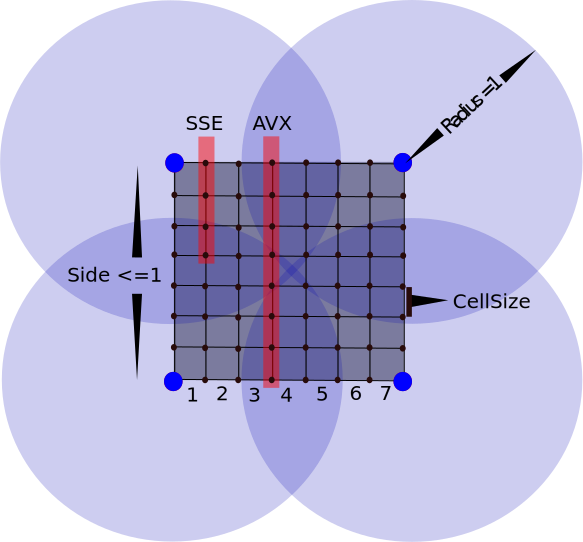
\includegraphics[width=0.9\linewidth]{figures/cpupoly/MPU.pdf}
  \caption{\label{fig:MPU}
  {The \textit{MPU} is our unit of computation per each core illustrated as a 2D cross section here. 
  Field-values due to every 4 or 8 points are computed in parallel with SSE or AVX instructions, respectively. 
  When the field at a vertex is zero no iso-surface will pass in the neighborhood of a unit circle (sphere in 3D) centered at that vertex.}
}
\end{figure}


\section{Algorithm}\label{sec:algorithm}
The input to our algorithm is a \blob data structure, representing an implicit model whose iso-surface we wish to find. Output is a 
triangle mesh.  The model bounding box and the cellsize parameter supplied by the user to control the resolution of the final mesh.
The \blob structure is first converted into a compact, linear structure required for SIMD optimization techniques, then the model 
bounding box is divided into the \textit{MPUSET} with respect to the \textit{cellsize} parameter.
The \textit{MPUSET} is processed in parallel using multiple cores; with a fast empty \textit{MPU} rejection method and SIMD surface 
extraction algorithm the mesh contained within intersecting $MPU$s is extracted. The algorithm has no synchronization points except after 
all \textit{MPU}s are processed and the triangle mesh is sent to the GPU for rasterization. The left column in figure 
(\ref{fig:AlgorithmHighLevelView}) displays these preparation steps in order.
The following sections describe this whole process in detail.


We start by describing the initialization phase and continue with the surface extraction details in the next section.
The algorithm starts by computing the size of an \textit{MPU} side (7 cells) and dividing the bounding box of the model into a 
3D grid of \textit{MPU}s, where each \textit{MPU} is assigned a unique global identifier. The main idea of our algorithm is parallel 
processing of the set of all \textit{MPU}s (\textit{MPUSET}) using multicore and SIMD processing techniques.

Our algorithm recursively splits \textit{MPUSET} into disjoint \textit{MPURANGE}s where each \textit{MPURANGE} is assigned to an idle core on 
the processor. The granularity of the divisions can be determined by the average amount of machine cycles spent to process an \textit{MPU}, 
however, in our implementation we resort to the solution provided by Intel Threading Building Blocks (TBB) \cite{Reinders2007}, 
which provides a non-preemptive task scheduling system to take care of the differences in task loads by 
monitoring processors and starting new tasks on idle cores automatically (work-stealing) \cite{Reinders2007}.


\begin{figure}[H]
  \centering
  % the following command controls the width of the embedded PS file
  % (relative to the width of the current column)
  \includegraphics[width=0.9\linewidth]{figures/cpupoly/AlgorithmHighLevelView}
  \caption{\label{fig:AlgorithmHighLevelView}
  {Left Column: The one-time preparation steps before scheduling kernel functions for computation.
  Middle Column: The early discard kernel function. Right Column: The $MPU$ processing kernel function.}
}
\end{figure}

\subsection{BlobTree Linearization}\label{sec:linearization}
The first step in our algorithm is the \blob reduction and pruning as suggested by Fox \etal \cite{Fox2001}.
In the second step, using the same linearization algorithm proposed for quadtrees \cite{Lee2000}; the \blob is converted into 
a pointerless representation to achieve cache-memory efficiency by keeping all input data structures at 
aligned memory addresses and fitting the entire \blob model into the last level cache memory of the processor. 
The final linearized \blob is in the format cache-line aligned structure of arrays. With this format several computations
can be optimized with SIMD instructions, e.g. applying a transformation matrix on a vector of 4 or 8 vertices as opposed to
scalar computation. The output mesh is also in the format of cache-line aligned structure of arrays which is the key to
compute colors and normals in SIMD fashion. 



\subsection{Surface Extraction}\label{sec:surfaceextraction}
In our algorithm we assign field values for every vertex of every \textit{MPU} that is not trivially rejected with the method explained in 
the following, and compute the triangular mesh representing the iso-surface. This approach combines elements of several algorithms 
(\cite{Wyvill1986, Lorensen1987, Bloomenthal1994a}).

We extended the method proposed by Zhang \etal \cite{Zhang2006} to trivially reject all empty \textit{MPU}s.
The observation made is that according to equation \ref{eq:WyvillFunc}, if the field value at a given vertex is zero then 
the shortest distance from that vertex to the iso-surface is greater than or equal to one (See figure \ref{fig:MPU}). Using 
this fact empty \textit{MPU}s can be identified very fast by evaluating the fields at the 8 vertices of each \textit{MPU} and rejecting it of all 8 
fields are zero. However, this test is only applicable when the cellsize parameter is smaller than or equal to $1/7$ or 0.1428. 
For larger \textit{cellsize}s the iso-surface may still intersect with the \textit{MPU} while the fields at vertices of the \textit{MPU} are zero. 
This process is depicted in the middle column of figure (\ref{fig:AlgorithmHighLevelView}).
For a discussion on \textit{cellsize} versus performance see section~\ref{sec:results}.

For larger \textit{cellsize}s we shoot 8 rays from the center of the \textit{MPU} to its eight vertices, using  the technique of Zhang \etal per 
each step we march $0.866c$ (0.866 is half of the diagonal of an \textit{MPU} with side one and $c$ being the cellsize parameter) along each ray. 
At each step we compute the fields for the 8 vertices along the rays; if a non-zero field is found then the \textit{MPU} is further processed, 
otherwise we march along the rays until we reach the vertices of the \textit{MPU}. 

If an \textit{MPU} is not rejected then it is further processed for surface extraction. A local copy of the linearized \blob is provided 
per each core in order to avoid \textit{false-sharing} among cores \cite{Bolosky1993}. Using SIMD processing techniques field values for all
512 vertices of \textit{MPU} are computed. With SSE or AVX instructions this step requires 128 or 64 field evaluation kernel runs, 
respectively (figure \ref{fig:MPU}).

All the fields are stored in a memory aligned array of 512 floating points. This technique avoids reevaluating field values while processing
cells in the next step. Storing field values from a SIMD register into memory aligned address can be accomplished with a SIMD instruction in
parallel. After this step all 343 cells of the \textit{MPU} are processed. Per each cell, the 8 vertex field values 
are gathered in SIMD fashion. Each vertex with a field greater than or equal to \textit{iso-value} is labeled one otherwise zero. 
The configuration index of the cell is computed using the SIMD method shown in algorithm \ref{alg:cellconfig}. A configuration index 
is computed to access the table as in \cite{Lorensen1987}. We used the modified marching cubes table proposed by Dietrich \etal that eliminates many 
of the degenerate triangles produced in the original MC algorithm \cite{Dietrich2009}. For the ambiguous cases we take another sample 
from the center of the cell \cite{Wyvill1986, Dietrich2009}. 

%bw - make this English
\begin{algorithm}[H]
\caption{SIMD computation of cell configuration. Pseudo code provided for AVX SIMD computation. Similar code can be written in SSE.}
\label{alg:cellconfig}
\begin{algorithmic}[1]	
  \STATE Gather the 8 vertex field values of the cell  
  \STATE simd $index = cmp\_ge8(fields, simd(0.5))$
  \STATE $index = and8(index, simd(1.0))$
  \STATE $index = mul8(index, maskPower)$  
  \STATE $index = hadd8(index, index)$   
\end{algorithmic}
\end{algorithm}

In algorithm (\ref{alg:cellconfig}) fields is an array of 8 vertex field values, 
line 2 performs a parallel comparison between \textit{iso-value} and fields. 
In line 4 maskpower shifts the field values into the appropriate slot in the SIMD array and finally line 5
performs a horizontal add operation on the values to compute the configuration index.

For each intersecting edge there is one inside and one outside vertex.
Using a root finding method the point of intersection of the iso-surface is computed and stored in a 
hash table to be reused by the neighboring cells that share that vertex. 

For the root finding methods that do not require gradient information such as regula falsi or bisection method, 
the field value should be evaluated multiple times along the edge, which will degrade the performance of the system. Other methods 
such as Newthon-Raphson require gradient information, and as mentioned in equation (\ref{eq:Normal})
each gradient computation involves 4 extra field evaluations. We describe a root finding
%%%  is this really new???/ 
technique based on SIMD instructions that computes the root with only one extra field evaluation in AVX (two with SSE) 
with adequate precision. By subdividing the intersecting edge into 8 vertices and evaluating the field values, the exact interval 
containing the final root can be identified. Performing linear interpolation in that interval will produce the 
final root (figure \ref{fig:root}), it is trivial to show when the number of intervals increases the interpolation error decreases \cite{Matthews1987}. 

\begin{figure}[H]
  \centering
  % the following command controls the width of the embedded PS file
  % (relative to the width of the current column)
  \includegraphics[width=0.8\linewidth]{figures/cpupoly/root.pdf}
  \caption{\label{fig:root}
  {Top: A cell edge is intersected with part of the surface shown in blue.  By performing one field evaluation using 
  AVX or two with SSE instructions the interval containing the intersection point can be identified. 
  The final root is computed using linear interpolation within the interval marked with bold line segment.}
}
\end{figure}


Algorithm (\ref{alg:surfaceextraction}) summarizes the process of surface extraction which is run per each \textit{MPU}. 
Lines 1 through 25 are related to the \textit{MPU} discard method explained earlier in this section. Lines 26 through 42
shows the cell processing technique which is optimized using SIMD cell configuration computation and our root 
finding method. Since color and normal attributes should only be computed for final mesh vertices, this step is 
performed last to fully leverage SIMD optimizations by performing every 4 or 8 attribute computations in 
one SIMD call which greatly enhances the throughput of the system and minimizes \blob traversals.

%%bw check this for undefined stuff - make ENglish
\begin{algorithm}
\caption{Algorithm for surface extraction of an \textit{MPU} using AVX SIMD instructions,
Similar code can be written for SSE instruction set. 
Input is linearized \blob $T$, lower vertex of \textit{MPU} and the \textit{cellsize} parameter. 
Output is the local mesh contained in the \textit{MPU}}
\label{alg:surfaceextraction}
\begin{algorithmic}[1]		
	\STATE $side \gets cellsize*7$
	\STATE simd $v \gets $Compute \textit{MPU} vertices
	\IF{$side \leq 1$}	
	\STATE simd $f \gets T.compute\_field8(v)$
	  \IF{$f == 0$}
	  \STATE return;
	  \ENDIF	
	\ELSE 
	  \STATE $flag \gets true$
	  \STATE $incr = 0.866*cellsize$	  
	  \STATE $d = incr$
	  \WHILE{$d \leq side * 0.866$}	
	  \STATE Shoot rays from center of \textit{MPU} to its 8 vertices
	  \STATE simd $v \gets $Travel along the rays for distance $d$     
	  \STATE simd $f \gets T.compute\_field8(v)$
	  \IF{$f != 0$}
	  \STATE $flag \gets false$
	  \STATE $break$;
	  \ENDIF
	  \STATE d = d + incr;
	  \ENDWHILE	
	  \IF{$flag == true$}
	  \STATE return;
	  \ENDIF	
	\ENDIF	
	
	\STATE float fieldCache[512];
	\FORALL{simd $vertex$ in $mpu$ vertices}
	\STATE simd $f \gets T.compute\_field8(vertex)$
	\STATE Store $f$ in appropriate location in $fieldCache$
	\ENDFOR
	
	
	\FORALL{$cell$ in $mpu$}
		\STATE $f \gets gather8(cell, fieldCache)$
		\STATE $edges \gets $Compute cell config from $f$ to access table
		\FOR{$i=1 \to $count of edges}
			\IF{root for $i$th edge is not stored in edge table}
			\STATE Compute and store root associated with $i$th edge		
			\STATE Add root to mesh vertices
			\ENDIF
		\ENDFOR				
		\STATE Add $cell$ triangles to mesh
	\ENDFOR	
	
	\STATE compute color and normal for all vertices (every 8 vertices in parallel)
\end{algorithmic}
\end{algorithm}


\section{Results}\label{sec:results}
We have implemented our algorithm using Intel threading building blocks in C++ on a Linux platform. We used two systems with 
different configurations. On the first system which has Intel i7-3960X processor with Sandy Bridge architecture, there are 6 
physical cores given that each core runs in hyper-threaded mode; up to 12 threads can run in parallel on this machine. 
This processor supports both SSE and AVX instructions and there is a last level cache memory of 15 megabytes 
which is shared between all cores.

The second system is a server with 4 Intel X7560 processor with Nehalem architecture. Each processor has 8 physical cores
or 16 in hyper-threaded mode and has 24 megabytes of last level cache memory and it does not support AVX instructions. 
Together these 4 processors provide us with as many as 32 physical cores (64 when hyper-threaded) on this server. 
We refer to these two systems with SNB and NHM respectively.


On the first experiment our goal was to prove the scalability of our algorithm. Figures (\ref{fig:PerfSNBTower}, \ref{fig:PerfXeonTower}) 
show the average running time of the algorithm when rendering towers model (figure \ref{fig:ModelTower}) on SNB and NHM systems, 
respectively. The \blob of the towers model has 7360 operators and 7296 primitives and a depth of 64 levels. 
In this test the cellsize parameter kept as a constant value of 0.14 which we found it to be a balance between number of triangles produced and 
the quality of the output mesh.  

In order to show the effect of SIMD optimizations we have tested our algorithm with scalar, 4-wide SSE and 8-wide AVX instructions. 
SSE being on average 4.58x faster than scalar and AVX being on average 7.35x faster than scalar run. As illustrated in figure \ref{fig:PerfSNBTower}
when the number of threads increases past 6, two threads run on every core; sharing hardware resources on the hyperthreaded cores.  
The slope is reduced because each thread gets less resources than it would if it ran alone on the core.  Past 12 threads, we 
schedule multiple threads per core, and they start to thrash the cache; making the algorithm memory bound.

Figure \ref{fig:PerfXeonTower} shows the performance of our algorithm when running on the NHM system. Doubling number of 
threads, doubled the performance of the algorithm on this machine up to 33rd thread. The same behavior is shown and hyper-threaded 
cores start to compete for memory access when having more than 32 threads running on this machine.

\begin{figure}[H]
  \centering
  \includegraphics[width = 1.0\linewidth]{figures/cpupoly/Perf_SNB.pdf}
  \caption{\label{fig:PerfSNBTower}
  {Average polygonization time of the towers model when running on SNB processor. Horizontal axis is the number of threads. 
  Vertical axis is time measured in milliseconds.}
}
\end{figure}

\begin{figure}[htb]
  \centering
  \includegraphics[width = 1.0\linewidth]{figures/cpupoly/Perf_NHM.pdf}
  \caption{\label{fig:PerfXeonTower}
  {Average polygonization time of the towers model when running on NHM processor. Horizontal axis is the number of threads. 
  Vertical axis is time measured in milliseconds.}
}
\end{figure}

%\begin{center}
\begin{table}[H]
\begin{center}
\caption{\label{table:speedup}{Comparison of speedups and field value evaluations per triangle (\textit{FVEPT}) for polygonization of Tower model 
  with different SIMD instruction sets. Note that FVEPT was 17 before adding SIMD optimizations.}}
  \begin{tabular}{ | l | c | c | c | }
    \hline    
    Processor & SIMD Method & Speedup & FVEPT \\ \hline \hline    
    SNB & SSE & 4.58x & 4 \\ \hline
    SNB & AVX & 7.35x	& 2 \\ \hline
    NHM & SSE & 4.25x & 4 \\    
    \hline
  \end{tabular}
  	
\end{center}
\end{table}
%\end{center}

Table \ref{table:speedup} shows the effect of using SIMD optimizations in our algorithm. With SSE and AVX the theoretical speedups are 4 and 8 times, 
respectively. Due to memory alignment techniques and proper caching mechanisms the speedup with 4-wide SSE is greater than 4. The AVX speedup can be 
improved more once scatter/gather instructions are implemented on the SNB processors which will improve the performance of surface extraction algorithm.
Number of field evaluations per triangle shows the average amount of times the field evaluation kernel called to compute a single vertex in the output mesh. 

In another experiment we studied the effect of our early discard method when the side of each \textit{MPU} is less than one 
(figure \ref{fig:DiscardEffect}). Starting from a large cellsize, we reduced the cellsize in uniform steps and measured the polygonization time. 
The red curve shows the polygonization time when the discard method described in section \ref{sec:surfaceextraction} is not being used and the blue curve 
is the timing when that method is in effect. Note that with the blue curve as soon as the \textit{MPU} side is less than one; (\textit{cellsize} = 0.14) empty 
\textit{MPU}s started to get discarded efficiently thus the constant part of the time value is reduced at that point.

\begin{figure}[htb]
  \centering
  \includegraphics[width = 1.0\linewidth]{figures/cpupoly/DiscardEffect2.pdf}
  \caption{\label{fig:DiscardEffect}
  {Reducing cellsize parameter results in more \textit{MPU} generation and increase in polygonization time.
  However, at a certain cellsize our early discard method stops polygonization time increase by rejecting 
  all empty \textit{MPU}s more efficiently.}
}
\end{figure}



%\ref{fig:ResultScaleSNBTower}, \ref{fig:ResultScaleXeonTower}
Figure \ref{fig:TowerSNBTimeBreakDown} shows the polygonization time breakdown when rendering the towers model on SNB processor. 
Horizontal axis is the core number for a total of 12 cores on that system. As can be seen from the top of this chart; 
the idle time is very short and the cores are active almost all the time. This shows that the work stealing algorithm scales well. 
190463 \textit{MPU}s are processed and 116723 of them are intersected with the iso-surface (40 percent were empty).
40 percent of the \textit{MPUSET} has been processed in less than 10 percent of the total polygonization time.

\begin{figure}[htb]
  \centering
  \includegraphics[width = 1.0\linewidth]{figures/cpupoly/PerCoreTimeBreakDown.pdf}
  \caption{\label{fig:TowerSNBTimeBreakDown}
  {Towers model per-core time breakdowns. Each bar represents a logical core on the processor for a total of 12 cores. 
  Vertical axis is the total polygonization time. 190463 \textit{MPU}s processed with 12 cores in 9283 milliseconds. 
  This chart shows the portion of time spent in each step of the algorithm when rendering the towers model on the 
  SNB processor with 8-wide AVX instructions.}
}
\end{figure}

\begin{figure}[htb]
  \centering
  % the following command controls the width of the embedded PS file
  % (relative to the width of the current column)
  \includegraphics[height = 0.8\linewidth]{figures/cpupoly/towers64}
  \caption{\label{fig:ModelTower}
  {Towers model created with skeletal primitives and binary operators in 
  our incremental designing system. The model is a grid of 8 by 8 towers for a total of
  7360 operators and 7296 primitives.}
}
\end{figure}

\begin{figure}[htb]
  \centering
  % the following command controls the width of the embedded PS file
  % (relative to the width of the current column)
  \includegraphics[width=0.7\linewidth]{figures/cpupoly/medusa}
  \caption{\label{fig:ModelMedusa}
  {Medusa model courtesy of Schmidt \etal \cite{SWG2005}.}
}
\end{figure}

These results demonstrate the scalability of our algorithm both in the number of SIMD vector lines and 
the number of cores available on each processor. 

Finally, we compare our method against Schmidt \etal's \cite{SWG2005} using the Medusa model provided by them   
which has 2920 primitives and 11 operators and the tree structure has a depth of 6 (figure \ref{fig:ModelMedusa}).
In this experiment, we divided polygonization timings reported in \cite{SWG2005} by 8 as the best AVX
optimized version of Schmidt's method. Then we ran our polygonization algorithm
optimized with AVX instructions on a single core for Medusa model (See table \ref{table:stats}). 

\begin{table}[H]
\begin{center}
	 \caption{\label{table:stats}
  {Comparison of our polygonization method against Schmidt \etal's \cite{SWG2005} 
  when rendering Medusa model at 5 different resolutions on one single core with AVX instructions. 
  All timings are in milliseconds.}
}
  \begin{tabular}{ | c | c | c | c |}
    \hline    
    CellSize & Our method & Schmidt's method & Speedup \\ \hline \hline
    0.01 & 5220 & 6228 & 1.19x\\ \hline
    0.03 & 3441 & 3653 & 1.06x \\ \hline
    0.05 & 1071 & 2175 & 2.03x	 \\ \hline
    0.10 & 264 & 1292 &	4.89x \\ \hline    
    0.14 & 108 & 721 & 6.67x \\        
    \hline
  	\end{tabular}
\end{center}
\end{table}


The results shows that our algorithm outperforms that of Schmidt \etal by a factor of 6 when running on a single core in lower resolutions. 

\section{Chapter Conclusions}\label{sec:futurework}
In this chapter we presented a new parallel polygonization algorithm using SIMD processing techniques that takes advantage of 
a multi-core machine. Our main contribution is a scalable algorithm both in terms of the number of cores available on 
multicore architectures and the number of SIMD vector width as shown in the results section.  We also presented a SIMD technique for 
finding the intersection of an iso-surface and a cube edge.

%\section{Acknowledgement}
%We would like to thank Intel Corporation for their support and providing us with their cutting-edge server and processors.
%This work is partly supported by the GRAND NCE foundation of Canada, and the Natural Sciences and Engineering Research Council of Canada.

	\startchapter{GPU discretization}
\label{chapter:GPUDiscretization}
In the previous chapter we presented an algorithm for polygonization of the \blob scene graphs on 
multi-core architectures. The output of that algorithm is a list of vertices with their associated attributes 
such as position, color and normal and a list of triangles that defines the connectivity of the surface mesh. 
While the surface mesh is used for rasterization it can also facilitate collision detection and contact 
modelling algorithms as we will see in the following chapters.  In this chapter we present an improved 
version of that algorithm that can take advantage of the processing capabilities of the GPU and provides 
scalable rendering performance on many-core architectures. 


Building on top of the results from our SIMD polygonization algorithm, in this chapter we present our 
work in optimizing that algorithm for many-core architectures such as GPU. The following are some of 
the reasons behind this effort:

\begin{enumerate}
 \item The polygonization process extracts a triangle mesh which ultimately requires rasterization for 
 rendering. Using a GPU implementation both steps can be fused together thus avoiding the expensive 
 read-backs. 

 \item GPUs provide a higher degree of SIMD processing which is also called SIMT for single instruction
 multiple threads. Using the same strategy, multiple units execute the same 
 fetched and decoded instruction; however, on the GPU side there is a wider access to 
 register sets, multiple flow paths and access to multiple memory addresses that can scale the 
 performance of each running thread significantly. 
  
 \item Using flexible and portable OpenCL programming, the polygonization code can be written 
 in simple, scalar arithmetic and the runtime environment will handle multi-threaded task 
 parallelism and vector width SIMD processing on the target hardware. This 
 is certainly much more readable and extensible code than using non-portable, machine 
 intrinsic functions for SIMD processing.
 
 
\end{enumerate}


When compared to the related work in the field, our proposed method has the following benefits:

\begin{itemize}
 \item It is dynamic, i.e., the input to our algorithm is a dynamic \blob structure that can change 
 in every frame. This is a key advantage that can enable interactive modelling sessions in an implicit 
 framework, i.e. the result of modifications to the model can be viewed in real-time. 
 After each change the associated meshes are updated dynamically. 

 \item It is high performance. The proposed GPU-based data-structure is compact enough to enable 
 rendering complex \blob models in the order of 60,000 nodes. (64,000 nodes only requires about 
 20MiB of video memory in our system).
\end{itemize}


The next section provides an overview on the design differences between a CPU and 
a GPU. Other considerations for memory and access patterns are discussed in that section.  
Next the data-structure and the new algorithm are explained. The chapter concludes with the results 
and analysis.

%Another requirement for the tetrahedral mesh generation is that the triangular surface mesh should be the boundary surface of the tetrahedral mesh. This is needed since 
%after applying the displacements to the volumetric tetrahedral elements the surface vertices should be displaced as well.
\section{Many-cores architectures}
One of the main differences between a multi-core CPU versus a many-core GPU 
architecture is the fact that the former is optimized for the fast execution of 
a single task by supporting a broad-set of instructions in hardware, where as the latter can accommodate 
heavy parallel processing in the format of single instruction multiple data (SIMD). 

CPU designers incorporate complex multi-cycle pipeline methodologies to amortize 
the amount of computation in a single machine cycle, e.g. by overlapping the execution of independent 
instructions at different cores, all cores of a processor are kept busy working on a different instruction. 
GPU designs take a different approach to parallelism. They achieve higher SIMD throughput by assigning 
more of the chip area to arithmetic logic units (ALUs) and less to fancy branch predictions and flow control. 
GPUs also have access to higher memory bandwidth when compared to their CPU counterparts.


The advent of programmable graphics pipeline opened up new avenues to exploit computational resources of the
GPU hardware. Before the introduction of general-purpose GPU (GPGPU) programming languages, such as open compute language (OpenCL), 
researchers in the field were forced to use computer graphics shading languages (e.g. glsl, cg) to gain access to 
the many-core architecture of GPUs. 

Many of the terms associated with solving rendering issues were borrowed to explain solutions to problems in 
other domains of science. Terms such as vertex, fragment and texture which define entities in a graphics 
shading problem were used to refer to the processing threads, work items and the input for a solution to a 
problem in high performance computing domain. In addition to the lack of a general language for computing on the GPUs, 
the complexity of mapping the problem domain to the graphics pipeline complicated the implementations and lead 
to various ad-hoc solutions to the same problems. For instance, Georgii \etal created an interactive cloth simulation 
by implementing a mass-spring system using fragment shader programming on an ATI X800 graphics card \cite{Georgii2005}. 
As another example S{\o}rensen \etal reviewed several shader programming techniques for accelerating 
linear system solving on GPUs with applications in surgical simulation \cite{Sørensen2006a}. 

At the time of this writing, the following languages are commonly used for GPGPU computing:
\begin{itemize}
 \item Nvidia CUDA (Compute Unified Device Architecture)
 \item Microsoft's DirectCompute
 \item OpenCL which is a standard language maintained by Khronos Group
\end{itemize}

Among all, OpenCL is the only language that is designed to be platform and 
host operating system independant, DirectCompute supports all hardware vendors
but is limited to Windows and CUDA is only available on Nvidia's hardware. 

OpenCL and CUDA share similar concepts in their programming model \cite{gaster2012heterogeneous}.
One of the major drawbacks of OpenCL when compared to CUDA is the initialization delay 
associated with the kernel compile process at runtime. The delay is significant for long
and complex kernels and at the time of this writing, no offline compiler is offered by Nvidia
to alleviate this issue. One way to improve this is to compile and store the binaries 
on disk upon the first kernel invocation and reuse the precompiled binaries for subsequent 
executions. 

The other technical issue that we faced with OpenCL is that the performance optimizations 
made on one platform are not transferred to other platforms. This situation has been experienced
by other researchers in the field and essentially there is no guaranteed portability for the 
tuning and optimizations of the kernels.
The algorithms that are presented in this chapter are implemented using OpenCL. 

OpenCL and CUDA use similar memory model to execute kernels on the GPU. Each thread of 
execution on the GPU has access to a limited amount of local memory that is private to that thread. 
The local memory for the thread is used to store the stack frames. It is also used in register spilling, 
which occurs when the local and private variables of the thread can not fit into the register file of the
physical core and they spill to the local memory. Each thread belongs to a thread block. In OpenCL terms 
a thread is referred to as a processing element and a thread block is called a compute unit. 

All processing elements within a compute unit has access to a shared memory block, which is 
accessible by all processing elements within the same block. Beside the local and shared memory
spaces, all processing elements have access to a global memory block which has the slowest access 
time when compared to the other two spaces. 

Physically, the local and shared memory spaces can be seen as level 1 and level 2 cache memory on the 
CPU and the global memory as the main memory (i.e. video memory on the GPU).



\section{Data Structures}
\label{sec:datastructure}
The \blob linearization step introduced in (section \ref{sec:linearization}) is modified to create a compact 
representation of the input model in our GPU polygonization algorithm. 

All the structures are aligned at 16 bytes (four floating points) memory addresses. This is similar to the texture 
accessing techniques in graphical shader programming languages such as GLSL or Cg, where four floats represent the 
RGBA values of a texel accordingly. If a primitive node has an associated transformation node with a non-identity 
transformation matrix, that matrix will be stored in the primitive matrices section of the input structure and an 
associated identifier (id) will be provided to the primitive. The inverse of the primitive matrix is computed 
and the first three rows are stored for further field computations. To transform the axis-aligned bounding 
boxes of the primitives, the full forward transformation matrix is stored in the box matrices section of 
the structure and it can be accessed using the same id provided for the primitive matrix.
Figure (\ref{fig:datastructure}) depicts this pointerless representation in details.

\begin{figure}[H]
  \centering
  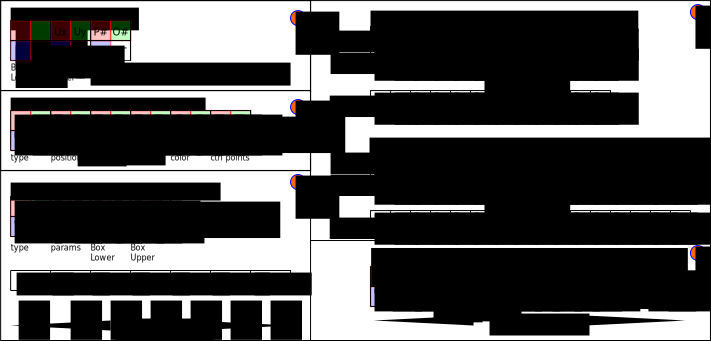
\includegraphics[width=1.0\linewidth]{figures/gpupoly/lineartree.pdf}
  \caption{\label{fig:datastructure}
  {The compact \blob scenegraph representation for GPU polygonization and tetrahedralization algorithms. The structure is 
  aligned at 16 bytes (4 floats). 1- The header. 2- Skeletal implicit primitives. 3- Operators. 4- Affine transformation 
  nodes. 5- Control points for sketched objects. Refer to section \ref{sec:datastructure} for details.}
}
\end{figure}

Each input data-structure is numbered in figure (\ref{fig:datastructure}) for further reference. We review the details in the following:
\begin{enumerate}
 \item The header section defines the lower and upper corner of the axis-aligned bounding box enclosing the entire model, 
 i.e. the convex hull of the input \blob. The header also contains the count of primitives, operators and the transformation 
 nodes. The id associated with the root operator of the tree is also defined in the header.
 
 \item The definition of each primitive is encoded in 6 texels. The $TP$ field in the first texel numerically encodes the 
 type of skeletal primitive. The other three fields in this texel are $MX$, $PR$ and $SB$ that link this primitive to its inverse 
 transformation matrix, the parent and the sibling elements respectively. The following texels define the position, 
 direction, skeleton-specific parameters and the color of the primitive. For the primitives that are 
 computed from sketched control points (e.g. the thin-plate spline primitives \cite{Turk1999, Grasberger}) the indices to the 
 associated first and last control points are stored in the last texel.

 \item A \blob operator is defined in 4 texels. Similar to the structure shown 
 in figure \ref{fig:linearized_blobtree}, links are provided to the child nodes.  
 Other fields added to support our stackless \blob traversal algorithm which is explained in the following 
 sections. The $NX$ field defines the next operator node in the \blob traversal route. 
 The $F^*$ field contains the flag bits that provide more control over the operator and the definition of 
 each can be found at the bottom of figure \ref{fig:datastructure}. Bits 1 and 0 are set in case the left child 
 or the right child of the current node are operators as well. Bit 2 is 
 set if the $LC$ and $RC$ indices are actually defining a range of indices for primitive children. If the unary 
 flag is set then the operator has only one child which is stored in the $LC$ field.  
 Bit 4 is set when the current operator appears as a right node for its parent. Bit 5 is the break route flag and is discussed further 
 in our stackless \blob routing algorithm. The rest of the bits are reserved for future use. 
 
 
 \item As mentioned above the inverse of the transformation matrices are computed and the first three rows are stored in our input 
 structure for field computation purposes. The elements are depicted in the format of [row][column]. The forward transformation is 
 stored as a 4x4 matrix in a separate input structure for performance reasons. 
 
 \item The control points associated with the sketched primitives are all stored in this section. Each control point is defined with 
 their XYZ coordinate and an associated weight value. 
\end{enumerate}

\section{Memory foot prints}\label{sec:memory}
After analyzing the performance of our OpenCL kernels, register spilling often found to be the major 
cause for many latencies. Resorting to shared memory spaces, reducing number of intermediate variables 
in field-evaluation kernels and avoiding loop unrolling in some cases helped to optimize the performance. 
Upon every change in the input \blob the linearized \blob is updated and transferred from main memory 
to the GPU. Currently the maximum number of nodes is set at 64K which covers all of the complex cases 
we modelled for this thesis. However, for larger \blob models we can easily increase this amount to 
support them. The memory footprint of our current \blob representation is summarized in table 
\ref{table:memfootprint}. Each row in the table represents a \blob with a specific number of nodes.
Starting from the simplest \blob with only one node (e.g. a sphere primitive) to the most complex \blob 
with one million nodes. The middle columns in the table are the break down of the required memory 
size per each component in the compacted \blob data structure.

\begin{table}[H]
\begin{center}
	 \caption{\label{table:memfootprint}
  {Memory footprint of the input \blob in our GPU polygonization algorithm in bytes. The entire \blob for a model with 64K nodes (primitives and operators) 
  takes up about 20 MiB in our current system.}
}
  \begin{tabular}{ | c | c | c | c | c | c | c | c |}
    \hline    
    Nodes & Header & Primitives & Operators & Prim Mtx & Box Mtx & Ctrl Points & Total \\ \hline \hline
    1 & 48 & 96/Prim & 64/Op & 48/Prim & 64/Prim & 16/Point & 320 \\ \hline
    1K & 48K & 96K & 64K & 48K & 64K & 16K & 320K \\ \hline
    64K & 3072K & 6144K & 4096K & 3072K & 4096K & 1024K & 20M \\ \hline
    1M & 48M & 96M & 64M & 48M & 64M & 16M & 320M \\ 
    \hline
  	\end{tabular}
\end{center}
\end{table}


\section{Stackless \blob traversal}
\label{sec:stackless}
As shown in figure \ref{fig:TowerSNBTimeBreakDown} the major bottleneck of the algorithm presented in chapter 
\ref{chapter:cpuPoly} is the surface extraction process. The expensive operations in that 
stage is the computation of normals and colors which require extra field evaluations and hence performance degradation. 

In this section we describe our novel stackless \blob traversal algorithm. 
Without a stack to be maintained the \blob traversal incurs less memory footprint. When dealing with small 
local memory available per thread on the GPU this reduction in memory usage improves the performance of the 
running kernels significantly. The idea behind the stackless traversal is to pre-compute a serial route to 
visit and evaluate all the operator nodes in the tree without using a global temporary storage to keep 
track of the visited nodes. An index based data structure is designed to provide sibling node access 
as well as two-way parent child relationships. This type of links help to perform horizontal and 
vertical moves in the tree structure.


In high performance rendering algorithms the use of hierarchical spatial data structures for acceleration reasons 
is common. Visiting nodes in such structures requires a stack-based depth-first search (DFS) traversal algorithm. 
Unfortunately, even the latest GPU architectures are poorly suited for implementing such algorithms. 

A complex \blob scene-graph data structure may contain thousands of primitives and operators which 
can lead to deep tree structures. Using the original DFS algorithm, the fieldvalue evaluation 
process has two stages: A ``down traversal'' followed by an ``up traversal''. 

During the down traversal stage all operators starting from the root node are visited and pushed onto an 
operators stack until a leaf node (primitive) is reached at which point the field due to the primitive is 
computed and pushed onto a separate fields stack and the next stage which is the up traversal begins.

During the up traversal stage the operators are popped out of the stack and per each child an associated field is popped from the fields stack for the 
operator to combine them in its own specific way. The resulting field is again pushed back on the fields stack.  This process continues until the 
operators stack get emptied and the final fieldvalue due to the root node is computed and returned.

Performing many push and pop operations limit the performance of the traversal process. The other issue 
relates to the inherently dynamic storage requirement for the stack itself. Although, creating a fixed-size 
stack is possible but since the stack size is a function of the number of nodes in the input, this will 
ultimately limit the maximum number of nodes in a complex scene. If $N$ is the maximum number of nodes 
(primitives plus operators) allowed in a \blob model then the minimum number of elements to be stored 
in the stack during the traversal process is equivalent to the depth of the tree. Implementing a stack in the 
global video memory will require very expensive memory transfers and is not an option for a real-time 
rendering algorithm. 

Our algorithm is based on the neighbor cell-links concept in the stackless traversal of spatial subdivision trees 
which is first introduced by Samet \etal \cite{Samet1984,Samet1990}. Using a similar technique Popov \etal presented 
a stackless KD-Tree traversal for high performance GPU ray tracing algorithm \cite{Popov2007}. 

The novelty of our technique is in the route computation and evaluation process which is completely 
different than what is proposed in Samet's and Popov's work. In our system, the geometry is not explicitly 
defined in the input structure at the time of route computation. Both Samet's and Popov's algorithms are 
based on spatial data-structures that provide explicit access to the geometry and therefore it is possible 
to recompute the missing sibling and parent-child relationships if they are not pre-computed. The 
second difference is the fact that not all the child nodes in  accelerator structures such as KD-Trees or 
BSP-trees need to be visited to answer an inclusion query, but in case of a \blob structure all nodes are 
visited in order to compute the final field due at a point in space. Once the field is computed then it is 
trivial to answer the inclusion query. A third difference is in the order of evaluating the operator nodes. 
Some operations such as difference, are not commutative and need a specific handling when computing 
the route. Such differences require special handling that clearly show the need for a different tree 
traversal algorithm.


The algorithm is divided into two stages. A preprocessing stage to compute a traversal route for the entire 
\blob and the GPU-based stackless traversal stage to compute the field-value due to a given point in space. 
The following will describe these two stages in greater details.


\begin{figure}[H]
  \centering
  % the following command controls the width of the embedded PS file
  % (relative to the width of the current column)
  \includegraphics[width=1.0\linewidth]{figures/gpupoly/stackless.pdf}
  \caption{\label{fig:stackless}
  {Stackless \blob traversal algorithm performs faster on deep tree traversals. The route is computed once and encoded into the tree upon transferring the input 
  data structures to the GPU.}
}
\end{figure}

\subsubsection{Encoding traversal route}
The first stage in our algorithm is to compute a route to visit all nodes in the \blob 
and finally encode that route in the GPU input data-structure. This process is performed only once and is not a 
bottleneck in the system. The one-time fixed cost paid for this stage on the CPU is regained 
when many fieldvalue evaluations are performed in parallel on the GPU without the extra cost 
associated with the stack storage.

To compute the route the following steps are performed on the CPU side as a preprocessing stage: 

Using the naive \blob traversal algorithm the nodes are visited from root to leaves. Two stacks are maintained in this process, an
operators stack $S1$ and a \text{break} nodes stack $S2$. The latter is defined in the following:

\begin{enumerate}
 \item If one of the children is an operator $A$ and the other is a primitive $B$. The parent for $A$ is set 
 to the current node and then it is pushed onto $S1$.
 
 \item If both children are operators. The right child is set as a \textit{break} node and is pushed on to $S2$. 
 The route at break nodes is flipped to the left branch of the tree, see figure \ref{fig:stackless}. 
 
 \item If the two children are both primitives: First the root of the \blob is set to the current node if it has not been set before.
  (Refer to the \blob header format in figure \ref{fig:datastructure} for the location of the root field shown as $RT$.) 
  A rope is created between the two primitives, linking the two nodes and a break node $B$ is popped from $S2$. 
  The next node for $B$ is set to the current node.
 
  
 \item This process is continued until $S1$ is emptied.
\end{enumerate}


%add an algorithm listing for this

%describe what happens on the GPU as well

\subsubsection{Up-sweep traversal on the GPU}
Figure \ref{fig:stackless}, shows the final route for a sample \blob. The benefits of this type of routing encoded into the tree
is that there is no need for storing a deep stack for the intermediate operators. Using this new approach the tree is now only evaluated 
from bottom to top. 

The \blob root node $RT$ marks the starting point of the traversal. This field is stored in the header section of the 
data structure as illustrated in figure \ref{fig:datastructure}. Using the new traversal route this field is set to
the operator node 10 for the example \blob shown in figure \ref{fig:stackless}. 

In case of an operator where all its children are primitives, the field due to each child is computed before the operator evaluation. 
The computed field is stored in the global field variable $F1$ and using the link to the next node provided in the structure ($NX$) 
the evaluation continues to the next operator in the tree at an upper level (up-sweep). When evaluating an operator with one primitive
child then the field due to the primitive child is computed before applying the current operator to $F1$ and performing the up-sweep (nodes 5 to 9 in 
figure \ref{fig:stackless}).

When visiting a break node the field is computed as usual but this time it is stored in the special variable $F2$, instead. 
In addition at a break node, the $NX$ field in the structure points to a non-parent operator (operator 4 for break node 3 in the example).

The process continues until the first node in the tree is evaluated at which the $F1$ and $F2$ values store the children fields for 
their parent. The $NX$ field associated with the first node points to itself which marks the end of the traversal process.


\section{GPU Surface Extraction Algorithm}
\label{sec:surfextraction}
In this section we present our GPU polygonization algorithm which is based on our novel field value evaluation technique described
in the previous section. Since the following steps are implemented using OpenCL on the GPU we will use the term \textit{kernel} which 
is a single thread of execution on the GPU. Please refer to section \ref{sec:memory} for a description of the memory model for
general purpose GPU (\textit{GPGPU}) programming.

We start by computing the axis-aligned bounding box of the model by traversing the tree from root to leaves 
and applying the transformation matrices at leaf nodes (primitives). Using the \textit{cellsize} parameter supplied by the user the 
bounding box is subdivided into a grid of voxels. The kernel \textit{ComputeAllFields} then computes a fieldvalue per each
vertex of the voxel grid and stores that value in the format of \textit{XYZF} where \text{XYZ} denotes the position and 
\textit{F} is the so-called field at that point. 


After computing all the fields, the grid edges are processed in the following order. 
Each vertex in the grid is connected to at most 6 other directly adjacent vertices. Starting from the lower corner of the voxel grid 
the kernel \textit{ProcessEdges} visits the corresponding vertex in the grid and examines only the edges that start 
from that vertex and extend to the adjacent vertices in the next index step. This way all edges in the voxel grid are checked 
and redundant traversals can be avoided. Needless to say that at boundary vertices the kernel may process less than 3 edges per each 
vertex (i.e. the ones that are within the convex-hull of the model). Upon each kernel run at this stage the index address to 
the corresponding vertex and its 3 other adjacent vertices is computed as shown in the algorithm \ref{alg:processedgeskernel}. Per each vertex
an inclusion query is performed (i.e. The fieldvalue at that vertex is compared against the iso-value. If it is greater than or equal 
the isovalue the vertex is considered inside otherwise outside the model). Two values are stored before completion of this kernel call. 
The first is the count of crossed edges at that vertex and the second one is a 3 bits flag which basically locates the intersected 
edges along x, y or z axes.


\begin{algorithm}[H]
\caption{\textit{ProcessEdges} kernel counts the number of intersected edges and their corresponding axes. 
This kernel runs per each vertex in the voxel grid.}
\label{alg:processedgeskernel}
\begin{algorithmic}[1]	
  \STATE $v = queryVertexInclusion(i, j, k)$
  \STATE $vx = queryVertexInclusion(i+1, j, k)$
  \STATE $vy = queryVertexInclusion(i, j+1, k)$
  \STATE $vz = queryVertexInclusion(i, j, k+1)$
  \STATE $count = (v \xor vx) + (v \xor vy) + (v \xor vz)$
  \STATE $flag = (((v \xor vx) << 2) or ((v \xor vy) << 1) or (v \xor vz))$
\end{algorithmic}
\end{algorithm}

In the above algorithm the \textit{queryVertexInclusion} function checks whether the vertex at a specified
voxel grid index is inside the model i.e. the field value at that vertex is greater than or equal to the \textit{isovalue}.
Then it performs the same test for the end-points of the edges emanating from the current vertex along the primary axes.
If both endpoints of an edges are inside (or outside) the model then there is no intersection between the iso-surface and
the voxel grid. Variable $count$ stores the number of intersections associated with the current vertex at the grid address 
$\left(i, j, k\right)$. In addition a 3 bits \textit{flag} variable holds the state of the intersections along the primary 
edges in the format of $XYZ$.

After processing all edges, the array \textit{EdgeBuffer} contains the count of intersected edges per each vertex 
in the voxel grid. In order to compute the total number of output vertices in the triangle mesh the prefix-sum 
\cite{Sengupta2007} of \textit{EdgeBuffer} is computed and stored in a separate gpu memory buffer called 
\textit{ScannedEdges}. The total number of vertices is the sum of the last elements in the \textit{EdgeBuffer} 
and \text{ScannedEdges} arrays. Before computing the vertex attributes such as the position, color and normal, the associated 
memory buffers are allocated on the device using the total number of vertices computed in the previous step. 

After this stage the vertex attributes of the mesh can be computed by executing a root finding method on the intersected 
edges and storing the output vertices in their appropriate buffer locations using the offsets in \textit{ScannedEdges}.
We use a Newton-Raphson root finding method which converges to the iso-surface using the gradient of the field \cite{Matthews1987}.
At each iteration the root is displaced closer to the surface according to the method given by Overveld \etal (\cite{VanOverveld2004}):

\begin{equation}
 r = r + \frac{\left(iso - f(r)\right)}{\nabla V(r).\nabla V(r)}
\end{equation}

Where $r$ is the root, $f(r)$ is the field at $r$ and $\nabla V(r)$ is the gradient of the field at $r$.
A maximum of four iterations was sufficient to provide smooth results in our tests. 
After computing the root position other attributes such as the color and normal at that vertex are also computed and stored in their 
designated buffers. The next step is to process the cells in the voxel grid in parallel and compute a configuration index per each cell
for extracting the topology of the triangles. There is no \blob traversal at this stage since the computed fields will be provided
to the kernel function. The configuration table is supplied as a texture and can be accessed using sampler unit for 
fast access. The number of triangles that are output per each cell is stored in a buffer called \textit{FaceBuffer}.

In order to find the total number of triangle elements, a prefix-sum scan is applied to the \textit{FaceBuffer} array 
in the same way that total number of vertices is computed previously. The buffer \textit{ScannedFaces} will be used to hold the 
offset values per each cell. 

The final stage in our GPU polygonizer is producing the triangles. For this purpose the kernel function \textit{GenerateFaces} 
is called per each cell in the voxel grid. No \blob traversal is required for this stage. Only the cells which intersect with the 
iso-surface are processed. Upon each kernel run the indices for the eight vertices of the current cell are computed. 

To process cell configurations we used the improved marching cubes table by Dietrich \etal 
\cite{Dietrich2009}, which avoids most of the small and badly shaped triangles. The table is supplied to the kernel as 
a texture of size 256 rows by 16 columns. To access the entries in the table the texture sampler on the hardware 
can be used. Per each cell the configuration index is computed using the previously stored fields. Each entry in the table is the 
index of an edge in the cell (There are 12 edges per each cell). Algorithm \ref{alg:generatefaceskernel} shows how the 
triangle elements are computed in this stage.

\begin{algorithm}[H]
\caption{\textit{GenerateFaces} kernel function computes the triangle indices per each cell and outputs them directly into an
OpenGL index buffer for rasterization. All the buffers can be read back from the GPU and stored.}
\label{alg:generatefaceskernel}
\begin{algorithmic}[1]	 
  \STATE $index = globalCellIndex(i, j, k, dim)$
  \STATE $config = cellconfig(i, j, k)$
  	  \IF{$config == 0$ or $config == 255 $}
	  \STATE return;
	  \ENDIF	
   \STATE $cellcorners = cellCornerIndices(i, j, k, dim)$
   \STATE $offset = ScannedFaces[index]$
   \STATE $count = FaceBuffer[index]$
   \FOR{$i=1 \to $count}
	 \STATE $edge = sample($configtable$, int2(edge, index))$
	 \STATE $start = EdgeStartIndex[edge]$
	 \STATE $axis = EdgeAxis[edge]$
	 \STATE $elements[offset + i] = ScannedEdges[cellcorners[start]] + axis$
   \ENDFOR				

\end{algorithmic}
\end{algorithm}


Upto five triangles can be extracted from each cell. Lines 11 and 12 in the algorithm assign the start index of an 
edge and its associated axis using two constant buffers supplied to the kernel for this purpose. 
The element entry is computed as an index to the global vertex buffer. The \textit{ScannedEdges} 
buffer holds the global offset for all the intersected edges as previously discussed. 

\section{Analysis and Results}
In this section we review the effects of the previous optimizations on the overall performance of the system.
In our experiments we tested the effect of the stackless \blob traversal algorithm using a set of models created 
with our incremental modelling system. To make a fair comparison the same algorithm implemented on the GPU using
the OpenCL framework once with the stack and the other time with the stackless method presented in section 
\ref{sec:stackless}. The results are shown in the following table:



\begin{table}[H]
\begin{center}
	 \caption{\label{table:stackless}
  {Stackless \blob traversal improved the performance of our \blob field evaluation significantly.
  Here is the comparison between our novel stackless approach versus the stack-based implementation for various models. 
  Timings are the average of 100 runs.}
}
  \begin{tabular}{ | c | c | c | c | c | c |}
    \hline    
    Model Name & Field Queries & Grid & Stack-based (ms) & Stack-less (ms) & Speedup \\ \hline \hline
    Tumor & 16240 & 29*20*28 & 21 & 0.8 & 26x\\ \hline
    cake & 18975 & 33*23*25 & 17 & 1 & 17x\\ \hline
    3slabs & 28750 & 46*25*25 & 30 & 2 & 15x \\ \hline
    \hline
  \end{tabular}
\end{center}
\end{table}


\begin{figure}[H]
  \centering
  % the following command controls the width of the embedded PS file
  % (relative to the width of the current column)
  \includegraphics[width=1.0\linewidth]{figures/gpupoly/combined_models.png}
  \caption{\label{fig:combinedmodels}
  {Sample models for testing our GPU polygonization method. From left to right: Cake, tumor and 3slabs.}
}
\end{figure}

When using stacks, the register spilling phenomenon mentioned previously degrades the performance due to the higher cost of accessing 
the shared memory. Conditional push and pops in the stack-based method also stalls the performance of the kernels.  

Faster field evaluations using the stackless algorithm also improves the performance of our root-finding method and the overall
polygonization time. In the following we review per kernel time break-time which provides a close look at hotspots (most time-consuming 
locations) in our implementation. 

%Tumor: Fields: 2, Edge: 1, EdgeBufferScan: 22, Vertex: 44, Cell: 1, FaceBufferScan: 18, Faces: 17, Total: 105
%Cake: Fields: 1, Edge: 1, EdgeBufferScan: 19, Vertex: 58, Cell: 2, FaceBufferScan: 17, Faces: 10, Total: 108
%3Slabs: Fields: 1, Edge: 1, EdgeBufferScan: 18, Vertex: 40, Cell: 1, FaceBufferScan: 17, Faces: 1, Total: 79

\begin{figure}[H]
  \centering
  % the following command controls the width of the embedded PS file
  % (relative to the width of the current column)
  \includegraphics[width=0.8\linewidth]{figures/gpupoly/breakdownpoly.pdf}
  \caption{\label{fig:breakdownpoly}
  {Polygonization time breakdown in milliseconds for the three models shown in the previous section. Vertex processing is the most compute-intensive
  stage due to the Newthon-Raphson root finding method employed and the evaluation of colors and normals which require additional traversals.
  }
}
\end{figure}

As it can be seen computing vertices is still the most time-consuming stage due to the extra tree traversals required for high quality 
gradiant-based Newthon-Raphson root-finding method. Computing other attributes such as colors and normals would also need 1 and 4 
traversals respectively. The prefix-sum scan operator employed here uses multi-pass computing. The extra cost of kernel calls has
increased the cost of using these operators. Several optimizations can be performed to benefit the overall performance. By 
vectorizing all kernels the core SIMD units can be used more efficiently. The prefix-sum scan operator can also be implemented in such a way 
that the memory-bank conflicts are completely avoided and the data-accesses are performed in parallel.























        \startchapter{Real-time Cutting}
\label{chapter:Cutting}
One of the main objectives of virtual reality based surgical simulation systems is the removal of pathologic tissue. 
	\startchapter{Evaluation, Analysis and Comparisons}
\label{chapter:evaluation}
During the past decade a new thrust has appeared with the development of tissue modelling techniques 
which could make it possible to develop patient-specific simulations. Whenever the best surgical strategy 
is unclear or the patient presents a rare pathology such simulations could be beneficial. Other use-cases for such systems is in surgical skill training which is a long 
and tedious process of acquiring fine motor skills. In all those scenarios physically-based animation of 
tissues is challenging and has lots of room for improvement. 

Our methods presented in the previous chapters have been integrated into our surgical simulation system. 
The result is a comprehensive environment for tissue modelling and simulation with support for cutting. 
We present our results in the context of a skull craniotomy procedure.

Craniotomy is a surgical operation in which a part of skull, called a bone flap is temporarily removed to access 
the brain. The operation is performed on patients with brain lesions, traumatic brain injury 
(TBI) or for brain biopsy purposes. Some treatment procedures are done by deep implantation of brain 
stimulators; Parkinson disease, epilepsy and cerebellar tremor are examples of such cases that require 
a craniotomy for the implantation process. 

Small dime-sized craniotomies are called burr holes or keyhole craniotomies. In 
order to precisely control surgical and biopsy instruments through these small holes, the surgeons 
frequently use image-guided computer systems or endoscopes. Burr holes or keyhole craniotomies are 
used for minimally invasive procedures to:

\begin{itemize}
 \item insert a shunt into the ventricles to drain cerebrospinal fluid (hydrocephalus)
 \item insert a deep brain stimulator to treat Parkinson Disease
 \item insert an intracranial pressure (ICP) monitor
 \item remove a small sample of abnormal tissue (needle biopsy)
 \item drain a blood clot (stereotactic hematoma aspiration)
 \item insert an endoscope to remove small tumors and clip aneurysms
\end{itemize}

In the following sections we review the previous work in this domain and then describe our experimental 
setup . The chapter concludes with results and analysis.

\section{Previous work}
Abe \etal fabricated plastic skull models of seven individual patients by stereolithography from three-dimensional
data based on computed tomography (CT) bone images \cite{Abe1998}. Surgical approaches and areas of craniotomy were 
evaluated using the fabricated skull models. They reported a better understanding of anatomic relationships, preoperative
evaluation of the proposed procedure and improved educational experiences for the residents and medical staff as the benefits of 
their system. They also reported that the time and cost of making such models are the main disadvantages of using them.

Wong \etal loaded patient specific CT scans of cranial bone and CT angiography of intracranial circulation
into the Dextroscope workstation supplied by Volume Interactions Pte. Ltd \cite{Wong2007}. They showed various 
use-cases of the zoom, rotate, move and crop functions of the Dextroscope to visualize various angles of 
positioning the craniotomy. However, their system does not provide a physically-based simulation of the procedure. 

Stadie \etal performed a study on the effectiveness of virtual reality systems for placing the craniotomies 
in minimally invasive procedures \cite{Stadie2011}.  They used the Dextroscope and RadioDexter workstations 
supplied by Volume Interactions Pte. Ltd. to visualize and annotate the 3D VR models. 
Those systems are also used to measure the curvilinear distances of the proposed craniotomy centers on the 
patients skull model but they can not perform a cutting procedure on the input VR models.

\section{Architectural constraints}
We are able to perform interactive cuts on a model with more than 60,000 cells. The GPU accelerated cutting algorithm 
presented in chapter \ref{chapter:Cutting} requires a modern GPU with OpenCL support. The system we used for this
experiment is equipped with an Nvidia Geforce GTX760 with 2GB of video memory and 1152 CUDA cores. The CPU is an 
Intel Core i7-4770K with 256 KB, 1MB and 8MB of L1 to L3 cache. This processor has 4 cores and up to 8 threads can run in parallel. 
Our system is also equipped with 16 GB of main memory. 

\section{Experiments}
In this section we review the experiments that are performed to evaluate the 
performance and quality of our cutting algorithm in the context of the Craniotomy procedure. 
In the first experiment we use an eggshell model that helps us to study the 
quality of the cut surfaces and the amount of time it takes to apply mesh modifications in the associated 
data-structures. Fewer finite element cells in the eggshell model helps us to isolate the mesh quality 
issues in the vicinity of the cut surfaces. 

Later we use the human skull model and drill multiple holes at different locations in the bone tissue.  
The location of the drills are chosen according to the recorded videos of various brain biopsy 
procedures. Beside the experiments with the drilling tool, the scalpel tool is also used for the visualization 
of the internal mesh cross-sections, which can be helpful in the study of scanned volume data-sets from 
arbitrary viewing angles. 

Our system also allows controlled cutting along the major axes. The main benefit of 
this feature is in studying the effects of vibrations and other hand movements when 
cutting models interactively, i.e. by comparing the axis-locked, controlled cutting to 
the same scenario with free-hand movements, one can investigate the effect of 
small vibrations along the cut trajectory and how it can lead to the generation 
of small and wedge-shaped elements in the volume mesh. 

\subsection{The Eggshell Model}
\label{sec:eggshell}
Before drilling an actual skull mesh with many tetrahedral elements we tested our system on a spherial model similar to 
an eggshell. This model is composed of 840 nodes and 2280 tetrahedral cells. The outer surface is composed of two layers 
of tetrahedral elements only (see figure \ref{fig:eggshell01}). To create this model implicitly a smaller sphere is subtracted 
from a larger one. 

\begin{figure}[H]
  \centering
  % the following command controls the width of the embedded PS file
  % (relative to the width of the current column)
  \includegraphics[width=0.7\linewidth]{figures/evaluation/eggshell01.png}
  \caption{\label{fig:eggshell01}
  {Eggshell model before being drilled by our cutting tool.}
}
\end{figure}

After the drilling operation, only 120 new elements are added to the mesh for a total of 2400 elements. The entire process is completed 
interactively. The small disjoint parts fall down on the ground due to gravity. Each disjoint part becomes an independent
deformable model in our system and subject to forces and deformations. Figure \ref{fig:eggshell02} left, shows the mesh after being 
drilled for the bare hole. In order to perform a stress test on the model 6 
holes are drilled in various locations of the eggshell model (see figure \ref{fig:eggshell02}, right).


\begin{figure}[H]
  \centering
  % the following command controls the width of the embedded PS file
  % (relative to the width of the current column)
  \includegraphics[width=0.4\linewidth]{figures/evaluation/eggshell02.png}
  \includegraphics[width=0.4\linewidth]{figures/evaluation/eggshell05.png}
  \caption{\label{fig:eggshell02}
  {Eggshell model after being drilled by our cutting tool. Left: The first drill, Right: 
  After drilling 6 holes to the model.}
}
\end{figure}

After completing this experiment successfully our algorithm showed to be robust enough to handle 
more complex meshes. In the next stage a real data-set of skull tissue is used for the craniotomy operation.

\subsection{Craniotomy}
\label{sec:craniotomy}
Fang \etal published a tetrahedral mesh data-set of the brain tissues \cite{fang2010mesh}. The MRI scanned data is 
segmented into the following four regions:

\begin{enumerate}
 \item Skull and scalp
 \item Cerebro-spinal fluid (CSF)
 \item Gray-matter
 \item White-matter
\end{enumerate}

The high-resolution version of these segments are not published at the time of this writing so we used the lower resolution 
which has enough details of the organ for our simulation scenarios. The data-set is converted from its original format 
(MATLAB mat file) to our volumetric mesh format. Table \ref{table:brainmesh} shows number of nodes, edges, faces and tetrahedral cells 
per each segment after the conversion process:

\begin{table}[H]
\begin{center}
\caption{\label{table:brainmesh}{Segmented brain data-set statistics.}}
  \begin{tabular}{ | l | c | c | c | c |}
    \hline    
     & skull & csf & gray matter & white matter \\ \hline \hline    
    Nodes & 14739 & 37136 & 50741 & 23737  \\ \hline
    Edges & 89681 & 181593 & 268300 & 126441 \\ \hline
    Faces & 141498 & 251823 & 384989 & 184536 \\ \hline
    Cells & 66554 & 107460 & 167528 & 81833 \\ \hline
    \hline
  \end{tabular}
\end{center}
\end{table}

Due to its stiff material properties the skull tissue is modelled as a rigid material in our simulation system. 
Figure \ref{fig:craniotomy01} shows the skull mesh in its initial position.

\begin{figure}[H]
  \centering
  % the following command controls the width of the embedded PS file
  % (relative to the width of the current column)
  \includegraphics[width=0.7\linewidth]{figures/evaluation/craniotomy01.png}
  \caption{\label{fig:craniotomy01}
  {The scene setup for the craniotomy operation.}
}
\end{figure}


The cutting tool in this scenario is a tube-shaped device which can drill into the skull tissue and separate the bone matter.
In our system, the tool is defined as a curve approximated by $N$ line segments. The tool movement is tracked in the space 
and the system checks for collisions between the tool and the model continuously. Figure \ref{fig:craniotomytube} shows the 
polygonal shape of the cutting tool while in contact with the skull tissue.

\begin{figure}[H]
  \centering
  % the following command controls the width of the embedded PS file
  % (relative to the width of the current column)
  \includegraphics[width=0.6\linewidth]{figures/evaluation/craniotomytube.png}
  \caption{\label{fig:craniotomytube}
  {Cutting tool is defined as a tube with a base composed of a curve approximated with $N$ line segments. 
  Collisions between the tool and the tissue are monitored constantly.}
}
\end{figure}

When in contact with the skull tissue the intersection of the side wall of the tool is computed against the edges of the 
skull model. With $N$ line segments the cutting tool has $N$ quadrilateral faces on its side wall, the edge intersection 
test is performed in our system by calling the kernel function given in algorithm \ref{alg:edgeIntersections} once per each quad.
After each call the hash-table storing the cut-edges is filled with the new cuts. 

The cutting configurations presented in section \ref{sec:cutconfigs} are extracted based on one intersection per edge, therefore
it's not possible to cut a given edge more than once. In our system we only accept the first cut-edge and this did not produce any 
visual defects. Perhaps a more robust implementation would be to approximate the cutting tool curve based on the size of the longest 
edge in the mesh. After the cutting is made the mesh is separated and each of the disconnected parts is converted into a separate node
in our scene-graph structure. This operation results in correct detection of the self-collisions in the subsequent frames of the simulation.

The internal gray, white and CSF matters are also included in this simulation. The drilling operation only affects the skull tissue and
in fact it does not pass the Dura layer. This condition is a requirement for the successful completion of this procedure. 

Figure \ref{fig:crosssection} shows the cross section view of the brain. The skull is cut with a scalpel tool 
to show the internal tissues which are drawn in blue for better visibility. 
\begin{figure}[H]
  \centering
  % the following command controls the width of the embedded PS file
  % (relative to the width of the current column)
  \includegraphics[width=0.5\linewidth]{figures/evaluation/crosssection.png}
  \caption{\label{fig:crosssection}
  {Cross section view of the brain layers. The skull shown in pink is cut using a scalpel avatar to show 
   all the other layers depicted in blue.}
}
\end{figure}


\begin{figure}[H]
  \centering
  \includegraphics[width=0.4\linewidth]{figures/evaluation/craniotomy06.png}
  \includegraphics[width=0.4\linewidth]{figures/evaluation/craniotomy07.png}
  \includegraphics[width=0.4\linewidth]{figures/evaluation/craniotomy09.png}
  \includegraphics[width=0.4\linewidth]{figures/evaluation/craniotomy10.png}
  \caption{\label{fig:craniotomy}
  {Simulation of the craniotomy operation using our surgical simulation framework with support for interactive cutting.}
}
\end{figure}

Figure \ref{fig:craniotomy} shows the operation (before, during and after drilling the first and the second holes). 
During the drilling process 845 and 940 tetrahedral cells are being cut in the vicinity of the drilling tool 
for the first and second holes, respectively. The interaction of the drilling tool and the skull 
was interactive at all times, supporting at least 60 frames per second.
        \startchapter{Conclusions}
\label{chapter:conclusion}
The following contributions were made:


\begin{enumerate}
  
\item A comprehensive modelling framework supporting a broad set of skeletal implicit primitives, 
 sketched primitive objects, warping, blending, affine transformations and constructive solid geometry 
 operators in the compact \blob structure. Our framework also provides a software architecture for 
 physically-based animation of rigid and deformable models.
 
 \item An algorithm for interactive polygonization of implicit surfaces on multi-core architectures with 
 SIMD instructions (peer reviewed). 
 
 \item An optimized GPU-accelerated algorithm for high-performance polygonization of implicit surfaces 
 on many-core architectures. 
 
 \item A novel mesh data-structure suitable for storing dynamic meshes on the GPU to support realtime 
 modifications during cutting
 
 \item Smooth, interactive cutting for complex elastic and rigid tissues 
 
% \item A novel technique for collision detection using implicit fields which is used in our system to detect 
%the intersection of the scalpel tool with the volume mesh in real-time. 
 
\item A real-time Craniotomy simulation for neurosurgery and biopsy simulations.

\end{enumerate} 

% 1. modelling framework
Our modelling framework enables physically-based animation of deformable models. 
This is better than what has been done by Cani \etal \cite{Grascuel1997}.  

% 2. SIMD polygonization method
Our SIMD polygonization method is peer reviewed \cite{Shirazian2012}. 
The proposed algorithm is scalable, dynamic and data-driven as opposed to the related work in this 
area where the input model can be either simple static functions or constant range data-sets 
\cite{Johansson2006, Tatarchuk2007, Knoll2007, Yang2010}.

% 3. GPU accelerated polygonization
Our proposed SIMD polygonization method is later optimized for using GPU acceleration. The 
proposed compact data-structure for \blob in section \ref{sec:datastructure} enables the transfer and 
rendering of large \blob in the order of 60,000 nodes interactively (as shown in that chapter using our 
compact data-structure a 64K nodes \blob only takes about 20 MB in video memory).  The result is a 
high performance polygonization method that enabled real-time updates in our incremental modelling 
system. This result is better than the work of \cite{Knoll2007, singh2010real} 
in rendering implicit models and the work of \cite{Yang2010, chochlik2012gpu} 
in polygonization techniques.

 
% 4. GPU based dynamic mesh
An intuitive volumetric mesh data-structure is proposed which is suitable for storing dynamic meshes on 
the GPU to support realtime modifications during cutting. Our cutting results show that the presented 
data-structure is more performant and can benefit the related work in this domain 
\cite{Wu2004a, Wu2005, Courtecuisse2010}.

% 5. cutting contribution how does it compare to previous work
Our proposed GPU-based data-structure enables real-time updates of the volumetric meshes upon 
cutting. Our cutting algorithm as shown in section \ref{sec:cutalg} is interactive for approximately 100,000 finite 
element cells. This is sufficient to cover many surgical scenarios. The resulting finite element 
cells are of high quality (the tetrahedral cells are not flat or wedge-shaped) as shown in section \ref{sec:cutres}. 
This is better than what has been done in the work of Courtecuisse \etal \cite{Courtecuisse2010}.
The cut edges are smooth, not jagged and a minimal amount of tetrahedral elements are 
created as the result of elements subdivision and this is better than the results published by Courtecuisse
\etal and Steinemann \etal \cite{Courtecuisse2010, Steinemann}. 


% 7. Craniotomy simulation
We presented a Craniotomy simulation based on our real-time cutting algorithm and the segmented 
brain data-set published by Fang \etal \cite{fang2010mesh}. 
%Although at this point we don't support haptic feedback but the simulation is well-received by one neurosurgeon at Stanford school of 
%medicine and Dr. Sandrine deRibaupierre from Western University. 
Given the large number of finite element cells in the brain mesh (around 100,000), our 
simulation still runs at interactive rates and the cutting output is smooth for a high-quality simulation 
as shown in section \ref{sec:craniotomy}. Colchester \etal used superimposed surface mesh for 
guiding a Craniotomy simulation \cite{Colchester1994}. Abe \etal used plastic skull models for 
training this procedure \cite{Abe1998}. To the best of our knowledge our proposed method is the only 
physically-based simulation for this specific procedure. 




\section{Future Work}
There are many areas in which the proposed system may be improved. The polygonization method 
introduced in chapter \ref{chapter:GPUDiscretization} can be further extended to support more 
complex implicit primitives such as skeletal curve primitives. Such primitives can be helpful in modelling 
vain and other tube-shaped tissues. Support for implicit decals as suggested in \cite{DeGroot2014} can help 
in creating realistically textured organs. 

Our cutting algorithm can also be extended to support progressive cuts. Progressive cuts can 
enhance the level of realism perceived in cutting. Also incorporating a fluid simulation will enhance the cutting 
scenario for simulating blood and CSF fluids in the brain. Procedural models such as L-Systems can be 
used to simulate the small blood vessels in the brain biopsy simulation. 

As computational power continues to increase, and optimization algorithms continue to improve, implicit 
surfaces are likely to play a much larger role in computer graphics. It is the sincere hope of the author 
that this research demonstrates what that role might be, and will encourage others to explore this domain.




	%\appendix
	%\include{chapters/appendix/chapter_app}

% The style of bibliography exemplified here is the "plain",
% normally used in science theses. This is shown
% by the entry {plain} below. Substitute the
% appropriate bibliography style. See also the
% PDF file "InformationOnBibliographyStyles" in this
% directory for more choices.

% The Bibliography file is a BibTex file named
% UVicThesis.bib and called below

	\TOCadd{Bibliography}
	\bibliographystyle{plain}
	\bibliography{PouryaLibrary}

\end{document}
